% !TEX root = main.tex
% Appendix. A: formal setup. B: executors. C: proofs of Theorems 1-3, with numerical checks.
% D: aligned structured Transformer learning. E: experiments and two-path proofs.
% F: reproducibility.
\providecommand{\reg}[1]{\ensuremath{\mathsf{#1}}}

\section{Formal setup}
\label{app:formal}

This section states the definitions and assumptions that the main text summarizes.

\paragraph{Losses and credit.}

\begin{definition}[Outcome and step losses]
\label{def:losses}
Let $\bm z_t(\bm\theta)\in\R^K$ be the state logits at the position that predicts $s_t$, and $\bm z_{\bm\theta}$
those at the answer position. The \emph{outcome loss} is $\Lout(\bm\theta)=\E[-\log\softmax(\bm z_{\bm\theta})_y]$, and $\bm y=\bm e_y$ is the one-hot answer.
Write $\ell_t(\bm\theta)=\E[-\log\softmax(\bm z_t(\bm\theta))_{s_t}]$. The first state prediction is a boundary case: the previous
count $s_0$ sits in the prompt rather than at the predicting position. The \emph{step loss} is therefore the teacher-forced
transition loss
\[
 \Lstep(\bm\theta)=\frac{1}{n-1}\sum_{t=2}^n\ell_t(\bm\theta),
\]
and $\Lstep^{\mathrm{all}}(\bm\theta)=\tfrac{1}{n}\sum_{t=1}^n\ell_t(\bm\theta)$ also includes $t=1$.
\end{definition}

With $\bm u=K^{-1}\bm 1$, the outcome credit functional is $\outcredit=\cred_{\bm y-\bm u}$ (\cref{def:credit}), and with the state-only
predictor $\bm q_s$ and the rule signal $\bm g_t$ of \cref{sec:credit}, $\rulecredit=\E_t\E[\langle\bm z_t,\bm g_t\rangle]$ with $t$ uniform on $\{2,\ldots,n\}$. At zero
attention scores the network is additive over positions (\cref{prop:network}(iii)), so every interaction among letters passes through the
scores; the \emph{score-mediated credit} is the credit of the score-dependent part $\mathbf J_{\mathrm{score}}=\Jz-\mathbf J^{[0]}$ of the Jacobian (\cref{eq:score-split}),
$\bigl\|\E[\mathbf J_{\mathrm{score}}^\top(\bm y-\bm u)]\bigr\|$.

\paragraph{Architecture and initialization.}

\begin{assumption}[Architecture]
\label{ass:arch}
A causal Transformer with two blocks of softmax heads and ReLU MLPs, learned token and position
embeddings, a learned relative position bias $\beta_{i-j}$ added to every attention score and initialized at zero, no
LayerNorm, any widths (residual $d_{\mathrm{res}}$, head $d_{\mathrm h}$, MLP $w$) and a linear readout $\mathbf V$;
every logit vector is $\bm z=\mathbf V\bm h$ with $\bm h$ independent of $\mathbf V$. A head may have a fixed, input-independent causal submask;
ordinary attention uses the full prefix.
\end{assumption}

\begin{assumption}[Initialization]
\label{ass:init}
\emph{Scale.} $\bm\theta_0=\initscale\tilde{\bm\theta}$ with $\initscale\le\initscale_0:=c\min(1,\frac{1}{N_b})$, where every weight matrix and embedding block of $\tilde{\bm\theta}$ has operator norm
at most $a_0$ and the value-token embeddings have smallest singular value at least $\embconst>0$.

\emph{Biases.} Every MLP bias satisfies $|\tilde b_m|\ge1$, and each MLP bias vector has norm at most $N_b$.

\emph{Neighbourhood.} We work on
$\initball=\{\bm\theta:\|\bm\theta-\bm\theta_0\|\le\ballradius\initscale,\ \beta=0\}$ with $\ballradius=\min(\frac{1}{8},\frac{\embconst}{4})$, where $\beta$ is the
relative position bias.
\end{assumption}

\begin{assumption}[Task]
\label{ass:task}
The task is counting modulo $K\ge2$ (\cref{def:task}), so $\mixrate<1$.
\end{assumption}

\paragraph{Constants and widths.} On $\initball$, no ReLU unit changes sign (\cref{app:network}). Constants $c,C>0$ depend only on $a_0$, $\embconst$, $K$
and the numbers of blocks and heads, never on the widths, $n$, $\initscale$ or the time. Fan-in-scaled initialization
satisfies \cref{ass:init} w.h.p.\ at every width, with $a_0$ bounded in terms of the largest block aspect ratio,
$\embconst\ge\tfrac{1}{2}$ and $N_b\le2\sqrt w$, provided the MLP biases are drawn with $|\tilde b_m|\in[1,2]$, which default
initializations (zero or small biases) do not do; at the executor width the aspect ratios are bounded, so the theorems
hold there with $n$-independent constants for $\initscale\le c\min(\mixrate,n^{-1/2})$ (\cref{rem:end-width}).

\paragraph{Parameters and training.}

\begin{assumption}[Training]
\label{ass:gd}
Full-batch gradient flow $\tfrac{d\bm\theta}{dt}=-\mathbf P\nabla_{\bm\theta}\mathcal L(\bm\theta)$ on $\Lout$ or $\Lstep$, where $\mathbf P$ is the orthogonal projection onto
the trainable parameter blocks, with the relative
position bias held at its zero initialization. \Cref{thm:outcome-end} drops this restriction and lets the bias train (\cref{lem:bias-uniform}).
\end{assumption}

\label{rem:norms}Parameters carry the Euclidean norm of the vectorized parameters (Frobenius on
each block). In \cref{thm:main,thm:separation} the relative bias is fixed at zero, which is what $\beta=0$ in $\initball$ and
\cref{ass:gd} encode, and $\bm\theta$ denotes the parameters other than $\beta$: the Jacobian $\Jz$, the gradients $\nabla_{\bm\theta}\mathcal L$ and
$\nabla_{\bm\theta}\cred$, and the Jacobian terms of \cref{prop:score-degree} are taken with respect to these parameters only. The step-credit bounds use uniform
zero-score attention through \cref{prop:network}(iv) and do not cover a trained bias. \Cref{thm:outcome-end} allows the bias to be
trained: its proof uses only the logit bounds, which hold for every $\beta$ (\cref{lem:bias-uniform}). The runs of \cref{tab:reach} also train it. The in-regime runs of \cref{app:exp-regime} have no relative bias.


\section{Exact two-block executors}
\label{app:architectures}

This section proves \cref{prop:represent}. An implementation of the construction is in the accompanying code repository.

\paragraph{Architecture.}
\label{app:construction}
\label{app:model}
Each block has three heads with $d_{\mathrm h}=2n+6$ (the number of positions) and one ReLU MLP of width $\max\{|\Sigma|,3K(n+1),2n+1\}$;
there is no LayerNorm:
\begin{align*}
 \bm h_i&\leftarrow \bm h_i+\sum_{h=1}^{3}\sum_{j\le i}\operatorname{softmax}_{j\le i}\Bigl(\tfrac{1}{\sqrt{d_{\mathrm h}}}(\mathbf W^{(h)}_Q\bm h_i)^{\!\top}\mathbf W^{(h)}_K\bm h_j\Bigr)\mathbf W^{(h)}_V\bm h_j,\\
 \bm h_i&\leftarrow \bm h_i+\mathbf W_{\mathrm{out}}\relu(\mathbf W_{\mathrm{in}}\bm h_i+\bm b_{\mathrm{in}}),\qquad \mathrm{logits}_i=\mathbf V\,\bm h_i .
\end{align*}

\paragraph{Registers.} The residual stream is the concatenation of one-hot registers
\[
 \underbrace{\reg{tl}}_{|\Sigma|}\ \underbrace{\reg{tv}}_{K}\ \underbrace{\reg{pos}}_{d_{\mathrm h}}\ \underbrace{\reg{qry}}_{|\Sigma|}\ \underbrace{\reg{match}}_{1}\
 \underbrace{\reg{prev}}_{K}\ \underbrace{\reg{mt}}_{1}\ \underbrace{\reg{cnt}}_{1}\ \underbrace{\reg{s0}}_{K}\ \underbrace{\reg{out}}_{K},
 \qquad d_{\mathrm{res}}=2|\Sigma|+4K+d_{\mathrm h}+3 .
\]
$\reg r[a]$ is coordinate $a$ of register $\reg r$, and $\mathbf E_{\reg a\leftarrow\reg b}$ copies $\reg b$ into $\reg a$.

\paragraph{Layout.} Token ids: letters $0,\ldots,|\Sigma|-1$, value $v\mapsto|\Sigma|+v$, then SEP, ``:'', EOS. Positions ($0$-indexed):
\[
\begin{array}{ll}
 \text{prompt} & s_0@0,\quad w^\star@1,\quad w_t@(1+t),\quad \mathrm{SEP}@(n+2)\\
 \text{step row} & s_t@(n+2+t),\quad ``{:}"@(2n+3),\quad s_n@(2n+4)\\
 \text{outcome row} & ``{:}"@(n+3),\quad s_n@(n+4)
\end{array}
\]
Position $i$ predicts the token at $i+1$: $n+1+t$ predicts $s_t$, and $n+3$ predicts $s_n$ in the outcome row.

\paragraph{Programs.} State arithmetic is modulo $K$.
\begin{center}\small
\fitwidth{\begin{tabular}{@{}lll@{}}
\toprule
 & step executor & outcome executor\\
\midrule
block 1, head 1 & \multicolumn{2}{l}{$\reg{qry}\leftarrow$ the query, at every letter}\\
block 1, MLP & \multicolumn{2}{l}{$\reg{match}\leftarrow b_t$}\\
block 2, head 1 & $\reg{prev}\leftarrow\widetilde s_{t-1}$ & $\reg{cnt}\leftarrow$ mean of $\reg{match}$ over the letters\\
block 2, head 2 & $\reg{mt}\leftarrow\reg{match}$ of letter $t$ & $\reg{s0}\leftarrow s_0$\\
block 2, head 3 & copy the last displayed count to the answer position & ---\\
block 2, MLP & $\reg{out}\leftarrow\mathrm{lookup}(\reg{prev},\reg{mt})$ & $\reg{out}\leftarrow\mathrm{lookup}(\reg{s0},\reg{cnt})$\\
\bottomrule
\end{tabular}}
\end{center}

\paragraph{Route and average.} Let $\Omega_n=\max\{16,3\log(8(n+3))\}$, $C_Q=\Omega_n\sqrt{d_{\mathrm h}}$, and let $\mathrm{src}(i)\subseteq\{0,\ldots,i\}$ be the source set
of position $i$ (a fallback $\{f\}$ where none is listed). Set
\begin{equation}
 \begin{gathered}
 (\mathbf W_K)_{j,\reg{pos}[j]}=1,\qquad (\mathbf W_Q)_{j,\reg{pos}[i]}=C_Q\ \ (j\in\mathrm{src}(i)),\\
 \tfrac{1}{\sqrt{d_{\mathrm h}}}(\mathbf W_Q\bm h_i)^\top \mathbf W_K\bm h_j=\Omega_n\,[j\in\mathrm{src}(i)] .
 \end{gathered}
 \label{eq:route}
\end{equation}
With $\mathbf W_V=\mathbf E_{\reg a\leftarrow\reg b}$, the head writes into $\reg a$ the average of $\reg b$ over $\mathrm{src}(i)$, up to the leak bounded below; $|\mathrm{src}(i)|=1$ is a
route and $|\mathrm{src}(i)|>1$ an average. A fallback $f>i$ gives uniform attention at a position with no supervised prediction.

\paragraph{Lookup.} For a count $s$ and a bit $b\in\{0,1\}$, use one unit per pair $(s',b')$ with
\[
 \mathrm{pre}_{s'b'}=[s=s']+[b=b']-\tfrac{3}{2}=\begin{cases}\tfrac{1}{2}&(s',b')=(s,b),\\\le-\tfrac{1}{2}&\text{otherwise},\end{cases}
\]
and output weights $2\bm e_{s'+b'}$:
\begin{equation}
 \textstyle\sum_{s',b'}2\,\bm e_{s'+b'}\relu(\mathrm{pre}_{s'b'})=\bm e_{s+b}.
 \label{eq:lookup}
\end{equation}

\subsection{Both programs are exact}
\label{app:exact}

\begin{proof}[Proof of \cref{prop:represent}]
\emph{Ideal routing} ($\Omega_n=\infty$). With $m=\sum_tb_t$ and $[m=a]=\relu(m-a+1)-2\relu(m-a)+\relu(m-a-1)$,
\begin{gather*}
 \reg{match}_{1+t}=2\textstyle\sum_{a\in\Sigma}\relu\bigl([w_t=a]+[w^\star=a]-\frac{3}{2}\bigr)=b_t,\\
 \reg{prev}_{n+1+t}=\bm e_{s_{t-1}},\qquad \reg{mt}_{n+1+t}=b_t,\qquad
 \reg{cnt}_{n+3}=n\cdot\tfrac{1}{n}\textstyle\sum_tb_t=m,\qquad \reg{s0}_{n+3}=\bm e_{s_0},\\
 \reg{out}_{n+1+t}=\sum_{j,\iota}\bm e_{j+\iota}\,2\relu\Bigl([s_{t-1}=j]+[b_t=\iota]-\frac{3}{2}\Bigr)=\bm e_{s_t},\\
 \reg{out}_{n+3}=\sum_{j,a}\bm e_{j+a}[s_0=j][m=a]=\bm e_{s_n}.
\end{gather*}
The test $[s_0=j]$ is applied by adding $(n+2)([s_0=j]-1)$ to each of the three pre-activations of $[m=a]$. The readout has weight $20$
on $\reg{out}$ for value tokens and weight $20$ on the relevant $\reg{pos}$ coordinates for ``:'' and EOS; all unused maps are zero.

\emph{Finite scores.} A row puts total weight at most $\omega^{\mathrm{leak}}_n$ outside its sources, where
\[
 \omega^{\mathrm{leak}}_n=(d_{\mathrm h}-1)e^{-\Omega_n}<\frac{2(n+3)}{(8(n+3))^3}=\frac{1}{256(n+3)^2}.
\]
Hence
\begin{gather*}
 |\reg{match}-b_t|\le2\omega^{\mathrm{leak}}_n,\qquad \|\reg{prev}-\bm e_{s_{t-1}}\|\le\omega^{\mathrm{leak}}_n,\qquad |\reg{mt}-b_t|\le3\omega^{\mathrm{leak}}_n,\\
 |\reg{cnt}-m|\le3n\,\omega^{\mathrm{leak}}_n,\qquad \|\reg{s0}-\bm e_{s_0}\|\le\omega^{\mathrm{leak}}_n .
\end{gather*}
At the step positions,
\[
 \mathrm{pre}_{s_t}\ge\tfrac{1}{2}-4\omega^{\mathrm{leak}}_n>0>\max_{a\ne s_t}\mathrm{pre}_a,\qquad \reg{out}_{s_t}\ge1-8\omega^{\mathrm{leak}}_n .
\]
At the answer position the errors add to $(4n+2)\omega^{\mathrm{leak}}_n<\frac{1}{192}$, and the three-ReLU test is $1$-Lipschitz, so
\[
 \reg{out}_{s_n}\ge1-(4n+2)\omega^{\mathrm{leak}}_n,\qquad \max_{a\ne s_n}\reg{out}_a\le(4n+2)\omega^{\mathrm{leak}}_n .
\]
With readout weight $20$ and $a^\star$ the gold token at a supervised position,
\[
 z_{a^\star}-\max_{a\ne a^\star}z_a\ge20\min\bigl\{1-8\omega^{\mathrm{leak}}_n,\ 1-2(4n+2)\omega^{\mathrm{leak}}_n\bigr\}>19 .
\]

\emph{Open neighbourhood.} Let $\mathcal P_n$ be the finite set of gold prefixes and supervised positions. By continuity there is
$r_{\mathrm{exec},n}>0$ with
\[
 \|\bm\theta-\bm\theta^\star\|<r_{\mathrm{exec},n}\implies\max_{P\in\mathcal P_n}\|\bm z_{\bm\theta}(P)-\bm z_{\bm\theta^\star}(P)\|_\infty<\tfrac{19}{2},
\]
so every greedy prediction is $a^\star$, and induction over the continuation gives the claim.
\end{proof}


\section{Proofs of \texorpdfstring{\cref{thm:main,thm:separation,thm:outcome-end}}{Theorems 1-3}}
\label{app:damping-proof}
\label{app:mainproofs}

The four proof blocks below establish contraction, network locality, the plateau, and step credit.

\subsection{Fourier contraction}
\label{app:C-fourier}
\label{app:assumptions}




(A1)--(A4) denote \cref{ass:arch,ass:init,ass:task,ass:gd}, and (A3$'$) a uniform start. Unless stated otherwise the query and the start
count are fixed. Constants $c,C$ depend only on $a_0,\embconst,K$ and the numbers of blocks and heads. Every bound stated on $\initball$ also
holds on $\initball'=\{\bm\theta:\|\bm\theta-\bm\theta_0\|\le2\ballradius\initscale,\ \beta=0\}$, whose relative radius is at most $\min(\frac{1}{4},\frac{\embconst}{2})$; there
$|b_m|\ge(1-2\ballradius)\initscale\ge\frac{3}{4}\initscale$ and $\sigma_{\min}(\mathbf E_{\mathrm{val}})\ge\frac{\initscale\embconst}{2}$. The only width-dependent threshold is $\initscale_0=c\min(1,\frac{1}{N_b})$.

\paragraph{The bias condition.}\label{rem:two-block-bias} The bias condition of (A2) fixes one ReLU pattern for all inputs on $\initball$. The AdamW runs violate it: at their initialization
($n=8$, MLP width $54$, $\initscale=0.02$, Gaussian biases), $10$ to $19$ of the $54$ units per block switch with the letters. Those
runs therefore lie outside the regime of the theorems; \cref{app:exp-regime} repeats the key measurements inside it.


\begin{lemma}[Gradient split]
\label{lem:gradient-split}
For every differentiable model, with $\outcredit(\bm\theta)=\E[\langle\bm z_{\bm\theta},\bm y-\bm u\rangle]$,
\[
 \nabla_{\bm\theta}\Lout=\underbrace{\E\bigl[(\Jz)^\top(\bm p-\bm u)\bigr]}_{\text{answer-independent}}-\underbrace{\nabla_{\bm\theta}\outcredit}_{\text{answer-dependent}},\qquad
 \nabla_{\bm\theta}\outcredit=\E\bigl[(\Jz)^\top(\bm y-\bm u)\bigr].
\]
\end{lemma}

\begin{proof}
The logit gradient of the cross-entropy is $\bm p-\bm e_y=(\bm p-\bm u)-(\bm y-\bm u)$.
\end{proof}

\paragraph{Conditioning on unseen letters.}
\label{app:target-spectrum}

\paragraph{Contraction.}\label{app:contraction} By \cref{eq:lambda}, $\mixrate^2=1-2p(1-p)(1-\cos\tfrac{2\pi}{K})$, and for $K=2$,
$\mixrate=|1-2p|$ and $1-\mixrate^2=4p(1-p)$. With $\alpha=e^{2\pi\mathrm i/K}$ and the Fourier multipliers
$\rho_j=1-p+p\alpha^j$, so that $\mixrate=\max_{j\ne0}|\rho_j|$, one unseen letter multiplies each nonconstant count
mode $\alpha^{js_t}$ by $\rho_j$, while one displayed transition keeps the innovation
\begin{equation}
 \E\bigl[\bigl|\alpha^{j s_t}-\rho_j\,\alpha^{j s_{t-1}}\bigr|^2\bigr]=1-|\rho_j|^2\ge1-\mixrate^2 .
 \label{eq:move-variance}
\end{equation}
In the Fourier basis of $\one^\perp$, $\operatorname{Cov}(\bm g_t)$ is diagonal with entries $\tfrac{1}{K}(1-|\rho_j|^2)=\tfrac{2p(1-p)}{K}\bigl(1-\cos\tfrac{2\pi j}{K}\bigr)$,
which gives \cref{eq:local-variation}.

\begin{lemma}[Conditional contraction]
\label{lem:target-contraction}
Assume (A3) and fix the start count and the query, so that the letters are independent. Let $\bm\xi=\bm y-\bm u$, $S\subseteq[n]$ and $\mathcal F_S=\sigma(w_t:t\in S)$. Then
\begin{equation}
 \bigl\|\E[\bm\xi\mid\mathcal F_S]\bigr\|^2=\frac{1}{K}\sum_{j=1}^{K-1}|\rho_j|^{2(n-|S|)}\le\Bigl(1-\frac{1}{K}\Bigr)\mixrate^{2(n-|S|)} .
 \label{eq:horizon}
\end{equation}
Hence for every square-integrable $\mathcal F_S$-measurable matrix $\mathbf H$ with $K$ rows,
 $\bigl\|\E[\mathbf H^\top\bm\xi]\bigr\|\le\mixrate^{n-|S|}\,\|\mathbf H\|_{L^2},\qquad \|\mathbf H\|_{L^2}:=\bigl(\E\|\mathbf H\|_F^2\bigr)^{1/2}.$ 
\end{lemma}

\begin{proof}
Write $s_n=s_0+\sum_tb_t$. The letters are independent, so for $j\ne0$
\[
 \E\bigl[\alpha^{js_n}\bigm|\mathcal F_S\bigr]=\alpha^{js_0}\prod_{t\in S}\alpha^{jb_t}\prod_{t\notin S}\E\bigl[\alpha^{jb_t}\bigr]=\alpha^{js_0}\,\rho_j^{\,n-|S|}\prod_{t\in S}\alpha^{jb_t},
\]
whose modulus is $|\rho_j|^{n-|S|}$. Parseval over the nonconstant modes $j=1,\ldots,K-1$ gives the identity, and $|\rho_j|\le\mixrate$ the bound.
The matrix bound follows from \cref{eq:horizon} by the tower property
and Cauchy--Schwarz.
\end{proof}

\paragraph{Sharpness.}\label{rem:tight} The $j=1$ term of \cref{eq:horizon} is $\frac{1}{K}\mixrate^{2(n-|S|)}$, and $\mathbf H=\E[\bm\xi\mid\mathcal F_S]$ attains the second bound up to the
factor $(1-\frac{1}{K})^{1/2}$, so the exponent $n-|S|$ is sharp for $0<\mixrate<1$.

\subsection{Transformer score expansion}
\label{app:model-spectrum}

The contraction estimate helps only if we can control how many letters a network term uses. Expanding the attention scores does
this without asking the entire output to depend on a small set: each term has its own set of letters, and terms with larger sets
are smaller near initialization.

\paragraph{Score expansion.} For $\zeta\in[0,1]$, let $\bm z(\zeta)$ be the network with every score $\psi_{il}$, in both blocks, replaced by
$\zeta\psi_{il}$. Then $\bm z(1)=\bm z_{\bm\theta}$, and for every integer $k_0\ge0$,
\begin{equation}
 \bm z_{\bm\theta}=\sum_{k=0}^{k_0}\bm z^{[k]}+\bm z_{\mathrm{rem}},\qquad
 \bm z^{[k]}=\frac{1}{k!}\frac{d^k\bm z}{d\zeta^k}(0),\qquad
 \bm z_{\mathrm{rem}}=\int_0^1\frac{(1-\zeta)^{k_0}}{k_0!}\frac{d^{k_0+1}\bm z}{d\zeta^{k_0+1}}(\zeta)\,d\zeta .
 \label{eq:score-split}
\end{equation}
$\mathbf J^{[k]}$ and $\mathbf J_{\mathrm{rem}}$ are the corresponding Jacobian terms. A term \emph{reads} the letters whose inputs it contains.

\begin{proposition}[Score count and letter support]
\label{prop:score-degree}
Fix the start state and the query. For $\bm\theta\in\initball$, $\Jz=\sum_{k=0}^{k_0}\mathbf J^{[k]}+\mathbf J_{\mathrm{rem}}$, and there is $\attconst$ such that:
\begin{enumerate}[label=(\roman*),leftmargin=*,itemsep=2pt,topsep=2pt]
\item $\mathbf J^{[0]}=\mathbf J^{[0]}_\emptyset+\sum_{t=1}^n\mathbf J^{[0]}_t$, where $\mathbf J^{[0]}_\emptyset$ reads no letter, $\mathbf J^{[0]}_t$ reads only $w_t$, $\sup\|\mathbf J^{[0]}_\emptyset\|_F\le C\initscale$ and
$\sum_t\sup\|\mathbf J^{[0]}_t\|_F\le C\initscale^2$;
\item for $k\ge1$, $\mathbf J^{[k]}=\sum_\nu\mathbf T_{k,\nu}$, where each $\mathbf T_{k,\nu}$ reads at most $2k+1$ letters and $\sum_\nu\sup\|\mathbf T_{k,\nu}\|_F\le C\initscale^2(\attconst\initscale^4)^k$;
\item $\sup\|\mathbf J_{\mathrm{rem}}\|_F\le C\initscale^2(\attconst\initscale^4)^{k_0+1}$.
\end{enumerate}
The same bounds hold for $\bm z^{[k]}$ and $\bm z_{\mathrm{rem}}$ with one more factor $\initscale$. Suprema are over inputs; constants do not depend on
$n$, $k$ or $k_0$.
\end{proposition}

$\attconst$ is fixed once, large enough for \cref{prop:score-degree,prop:network}; it depends only on $a_0$, $\embconst$ and $K$.

\label{app:network}

\begin{proposition}[Bounds for the score expansion]
\label{prop:network}
Assume (A1)--(A2). Uniformly on $\initball$, at every position and input, with $\bm x_i$ the token-plus-position vector,
all derivatives with respect to $s$ are evaluated at $s=0$ along $\bm\theta+sv$.
Let $\|F\|_{\mathrm{abs}}$ be the absolute sum of $F$ at $\zeta=0$: expand $F$ into monomials, products of
parameter blocks, inputs $\bm x_j$ and input-independent attention weights; bound each monomial by the product of the norm bounds of its
parameter factors on the ball, of $\sup\|\bm x_j\|$ for its inputs, and of its weights; and sum these bounds before any cancellation:
\begin{enumerate}[label=(\roman*),leftmargin=*,itemsep=3pt,topsep=4pt]
\item with input-independent offsets $\bm O^1=\bm o_1$, $\bm O^2=\bm o_1+\bm o_2$: $\bm h_i^\ell=\bm x_i+\bm O^\ell+O(\initscale^2)$, $|\psi_{il}|\le C\initscale^4$,
$\|\bm z_i\|\le C\initscale^2$, $\|\dd{\bm z_i}{s}\|\le C\initscale\|v\|$;
\item for $k\ge1$, $\zeta\in[0,1]$ and $\|v\|=1$,
\[
 \frac{1}{k!}\Bigl\|\frac{d^k\bm z_i}{d\zeta^k}\Bigr\|\le C\initscale^3(C_0\initscale^4)^k,\qquad
 \frac{1}{k!}\Bigl\|\dd{}{s}\left(\frac{\mathrm d^k\bm z_i}{\mathrm d\zeta^k}\right)\Bigr\|\le C\initscale^2(C_0\initscale^4)^k;
\]
the same holds for the absolute sums at $\zeta=0$, for $\bm h^2_i$ with one power of $\initscale$ fewer, and for the Taylor remainder with $k=k_0+1$;
\item the zero-score network is affine in the inputs; its transported logit terms have tangent $O(\initscale^2)$, and direct-input and
input-free terms have tangent $O(\initscale)$; an order-$k$ coefficient contains at most $2k+1$ inputs; a one-score logit term has size
$O(\initscale^7)$ and tangent $O(\initscale^6)$;
\item with full-prefix attention, the terms of the order-$k$ coefficients at $\zeta=0$ that contain an earlier input $\bm x_l$, $l<i$, obey the
bounds of (ii) multiplied by
\begin{equation}
 \kappa_{l,i}=\frac{1}{m_i}\Bigl(1+\sum_{l<j\le i}\frac{1}{m_j}\Bigr),\qquad m_i=i+1,
 \label{eq:dilution}
\end{equation}
after enlarging $C_0$.
\end{enumerate}
The constants do not depend on $n$, the widths or $k$.
\end{proposition}

\begin{proof}
For a network quantity $F$ let $F^{[k]}(\zeta)=\frac{1}{k!}\frac{d^kF}{d\zeta^k}(\zeta)$, so that $\bm z^{[k]}=\bm z^{[k]}(0)$, and write $\|F^{[k]}\|$ for its supremum over
inputs, positions and $\zeta\in[0,1]$ (the $\ell_1$ norm for attention rows).

\emph{(i).} $|b_m|\ge\frac{3}{4}\initscale>C\initscale^2\ge|(\mathbf W_{\mathrm{in}}\bm h)_m|$, so one activation matrix $\mathbf D_{\mathrm{act}}$ serves every input and every $\zeta$, and
\[
 \begin{aligned}
 \bm h_i^\ell&=\mathbf M_\ell\bigl(\bm h_i^{\ell-1}+\bm a_i^\ell\bigr)+\bm o_\ell,\\
 \mathbf M_\ell&=\mathbf I+\mathbf W^\ell_{\mathrm{out}}\mathbf D_{\mathrm{act}}\mathbf W^\ell_{\mathrm{in}},\qquad
 \bm o_\ell=\mathbf W^\ell_{\mathrm{out}}\mathbf D_{\mathrm{act}}\bm b^\ell.
 \end{aligned}
\]
with $\bm a_i^\ell=\sum_{\mathrm{heads}}\sum_{j\le i}\omega_{ij}\mathbf W_V\bm h^{\ell-1}_j$ and $\omega_{i\cdot}=\softmax(\zeta\psi_{i\cdot})$. Then
 \[
\begin{gathered}
\|\mathbf M_\ell-\mathbf I\|\le C\initscale^2,\\ \|\bm o_\ell\|\le CN_b\initscale^2\le C\initscale,\\ \|\dd{\bm o_\ell}{s}\|\le(a_0+2N_b)\initscale\le C,
\end{gathered}
\] 
and $\|\omega_{i\cdot}\|_1=1$. Induction over the two blocks gives (i).

\emph{Softmax calculus.} Let $\omega=\softmax(s)$ and
$\E_\omega[f]=\sum_j\omega_jf_j$. For a direction $\bm\nu$,
\begin{align*}
 \left.\dd{}{t}\omega_j(s+t\bm\nu)\right|_{t=0}
 &=\omega_j(\nu_j-\E_\omega[\bm\nu]),\\
 \left.\dd{}{t}\E_{\omega(s+t\bm\nu)}[f]\right|_{t=0}
 &=\E_\omega[\bm\nu f]-\E_\omega[\bm\nu]\E_\omega[f].
\end{align*}
After $k$ derivatives, each term has at most $k+1$ differentiable factors
and contains each direction once. The absolute coefficient sums satisfy
$a_{k+1}\le2(k+1)a_k$, $a_0=1$. Summing against the probability weights gives
\begin{equation}
 \bigl\|D^k\omega(s)[\bm\nu_1,\ldots,\bm\nu_k]\bigr\|_1\le2^kk!\prod_a\|\bm\nu_a\|_\infty .
 \label{eq:softmax-avg}
\end{equation}
For the smooth finite-dimensional maps in the fixed-ReLU region, the
higher-order chain rule \citep[Theorem~2]{clark2013faa} yields
\[
 \frac{1}{j!}\|D^jF\|\le Ac^j,\quad \|h^{[k]}\|\le ab^k
 \quad\Longrightarrow\quad
 \|(F\circ h)^{[k]}\|\le Aca\,b^k(1+ca)^{k-1},\quad k\ge1.
\]
Here the inner map's derivative bounds hold for every positive order; the
composition count is $\binom{k-1}{j-1}$.

\emph{(ii), values.} With $\|\bm\omega^{\ell,[0]}\|_1=1$, $\|\bm h^{0,[k]}\|=0$ for $k\ge1$, and $a_r\ge1$ in the compositions,
\begin{alignat*}{2}
 \|\psi^{\ell,[k]}\|&\le C\initscale^2\textstyle\sum_{a+b=k}\|\bm h^{\ell-1,[a]}\|\,\|\bm h^{\ell-1,[b]}\| &\qquad& \why{score is a product}\\
 \|(\zeta\psi^\ell)^{[k]}\|&\le\|\psi^{\ell,[k]}\|+\|\psi^{\ell,[k-1]}\| && \why{$(\zeta\psi)^{[k]}=\zeta\psi^{[k]}+\psi^{[k-1]}$}\\
 \|\bm\omega^{\ell,[k]}\|_1&\le\textstyle\sum_{j=1}^k2^j\sum_{a_1+\cdots+a_j=k}\prod_r\|(\zeta\psi^\ell)^{[a_r]}\| && \why{composition, \cref{eq:softmax-avg}}\\
 \|\bm a^{\ell,[k]}\|&\le C\initscale\textstyle\sum_{a+c=k}\|\bm\omega^{\ell,[a]}\|_1\,\|\bm h^{\ell-1,[c]}\| && \why{head output is a product}\\
 \|\bm h^{\ell,[k]}\|&\le C\bigl(\|\bm h^{\ell-1,[k]}\|+\|\bm a^{\ell,[k]}\|\bigr) && \why{affine block}\\
 \|\bm z^{[k]}\|&\le C\initscale\,\|\bm h^{2,[k]}\| && \why{readout}
\end{alignat*}
With $b=C\initscale^4$, block $1$ gives, for $k\ge1$, $\|\bm\omega^{1,[k]}\|_1\le b^k$ and $\|\bm a^{1,[k]}\|+\|\bm h^{1,[k]}\|\le C\initscale^2b^k$ (while $\|\bm h^{1,[0]}\|\le C\initscale$). Then $\|\psi^{2,[0]}\|\le C\initscale^4$,
$\|\psi^{2,[k]}\|\le C\initscale^5(k+1)b^k$ for $k\ge1$, and $\|(\zeta\psi^2)^{[k]}\|\le C(2b)^k$, so
\begin{gather*}
 \|\bm\omega^{2,[k]}\|_1\le C\sum_{j=1}^k\binom{k-1}{j-1}C^j(2b)^k\le C(Cb)^k,\\
 \|\bm a^{2,[k]}\|+\|\bm h^{2,[k]}\|\le C\initscale^2(Cb)^k,\qquad \|\bm z^{[k]}\|\le C\initscale^3(C_0\initscale^4)^k .
\end{gather*}

\emph{(ii), tangents, remainders, absolute sums.} Differentiating along $v$ replaces one factor of each product by its tangent, or one
$(\zeta\psi)^{[a]}$ in a softmax term, or adds $D^{j+1}\omega[\dd{(\zeta\psi)^{[0]}}{s},\ldots]$. With $\|\dd{\bm h^{0,[0]}}{s}\|=O(1)$, $\|\dd{\psi^{\ell,[0]}}{s}\|=O(\initscale^3)$
and $j+1\le2^k$ absorbed into $C_0^k$,
\begin{gather*}
 \|\dd{\bm\omega^{\ell,[k]}}{s}\|_1\le C\initscale^{-1}(C_0\initscale^4)^k,\qquad \|\dd{\bm a^{\ell,[k]}}{s}\|+\|\dd{\bm h^{\ell,[k]}}{s}\|\le C\initscale(C_0\initscale^4)^k,\\
 \|\dd{\bm z^{[k]}}{s}\|\le C\initscale^2(C_0\initscale^4)^k .
\end{gather*}
The integral remainder is bounded by the supremum of the next normalized derivative.

\emph{Absolute sums.} $\|\cdot\|_{\mathrm{abs}}$ is subadditive and submultiplicative, and $\|F\|\le\|F\|_{\mathrm{abs}}$. At $\zeta=0$ every attention row is an
input-independent probability vector $\bm\pi$ (uniform over the visible sites here, $\softmax(\beta)$ in \cref{lem:bias-uniform}), and
 $\Bigl\|\textstyle\sum_j\pi_j\prod_rF_r(j)\Bigr\|_{\mathrm{abs}}\le\prod_r\max_j\|F_r(j)\|_{\mathrm{abs}} .$ 
At $\zeta=0$, $D^j\omega$ expands as $\omega(0)$-weights times products of direction entries and $\omega(0)$-averages, with total coefficient at most $2^jj!$,
so \cref{eq:softmax-avg} holds for absolute sums with $\|\bm\nu_a\|_\infty$ replaced by $\max_l\|\nu_{a,l}\|_{\mathrm{abs}}$. Hence every line of the recursion
above holds verbatim for $\|\cdot\|_{\mathrm{abs}}$ at $\zeta=0$, which gives the absolute-sum bounds of (ii).

\emph{Tangents of absolute sums.} Take the norm bound of every parameter factor at least $\initscale$ (weights and embeddings $(a_0+1)\initscale$,
biases $(N_b+1)\initscale$). An order-$k$ monomial has at most $C(k+1)$ factors: at most $k$ scores, each with $\mathbf W_Q$ and $\mathbf W_K$, and at
most $2k+1$ inputs, each carried by at most four parameter blocks. Replacing one factor by its unit-direction tangent multiplies the bound by at
most $\frac{1}{\initscale}$, so the tangent bound is at most $\frac{C(k+1)}{\initscale}\le\frac{C2^k}{\initscale}$ times the monomial bound, uniformly in the unit direction
$v$; this lets $\sup_v$ pass inside the sum over monomials.

\emph{(iii).} At zero scores the network is affine in the inputs (for a head with a submask, $\frac{1}{m_j}$ becomes one over the size of its
visible set):
\begin{gather*}
 \bm h^1_j=\mathbf M_1\Bigl(\bm x_j+\frac{1}{m_j}\sum_{l\le j}\mathbf W^1_V\bm x_l\Bigr)+\bm o_1,\\
 \bm z^{[0]}_i=\mathbf V\Bigl[\mathbf M_2\Bigl(\bm h^1_i+\frac{1}{m_i}\sum_{j\le i}\mathbf W^2_V\bm h^1_j\Bigr)+\bm o_2\Bigr].
\end{gather*}
Transported terms contain $\mathbf V$, $\mathbf W_V$ and some $\bm x_j$, so their tangent is $O(\initscale^2)$; direct-input and input-free terms have tangent $O(\initscale)$.
With $d(F)$ the number of input occurrences in $F$,
\begin{alignat*}{2}
 d(\bm h^{\ell,[a]})&\le2a+1 &\qquad& \why{induction on $\ell$}\\
 d(\psi^{\ell,[b]})&\le2b+2 && \why{score is a product of two residuals}\\
 d\bigl((\zeta\psi)^{[a]}\bigr)&\le2a && \why{$(\zeta\psi)^{[a]}=\psi^{[a-1]}$}\\
 d(\text{order-$k$ head term})&\le2a_1+\cdots+2a_j+2c+1=2k+1 && \why{$a_1+\cdots+a_j+c=k$}
\end{alignat*}
and affine MLPs and parameter derivatives add none. The one-score correction is
 $\frac{1}{m_i}\sum_{j\le i}\bigl(\psi_{ij}(0)-\bar\psi_i(0)\bigr)\mathbf W_V\bm h_j(0),\qquad \bar\psi_i(0)=\frac{1}{m_i}\sum_{l\le i}\psi_{il}(0);$ 
its logit terms contain $\mathbf V,\mathbf W_V,\mathbf W_Q,\mathbf W_K$ and three residual inputs, so they have size $O(\initscale^7)$ and tangent $O(\initscale^6)$.

\emph{(iv).} Fix $l<i$; (iv) concerns the coefficients at $\zeta=0$ and their tangents. Replace $\bm x_l$ by $u\bm x_l$. A monomial containing $\bm x_l$
exactly $d\ge1$ times carries $u^d$, so
 $\sum_{\term\ni\bm x_l}\|\term\|_{\mathrm{abs}}\le\frac{d}{du}\Bigl(\sum_{\term}\|\term\|_{\mathrm{abs}}\Bigr)\Big|_{u=1},$ 
a tangent along an input direction, which obeys the product and composition rules above. Call $I^{(\ell)}_j$ a weight of position $j$ if every
marked order-$k$ coefficient of $\bm h^\ell_j$ (absolute sum and tangent) is at most $I^{(\ell)}_j$ times the unmarked bound of (ii); then
$I^{(0)}_j=\mathbf 1[j=l]$. At $\zeta=0$, $\omega_{jj'}=\frac{1}{m_j}$, and each term of a $\zeta$-derivative of $\omega_{jj'}$ is $\omega_{jj'}$ times score entries and
$\E_\omega$-averages, so each entry of an order-$a$ row coefficient is at most $\frac{1}{m_j}$ times the bound \cref{eq:softmax-avg}, which stays
valid with one $\|\bm\nu\|_\infty$ replaced by $\E_\omega|\bm\nu|$. A marked factor of the head output at $j$ contributes:
\[
\begin{array}{@{}lll@{}}
 \text{Marked factor} & \text{Weight} & \text{Reason}\\[2pt]
 \text{value at }j'\le j & \frac{1}{m_j}I^{(\ell-1)}_{j'} & \text{entrywise row bound}\\[2pt]
 \text{key at }j'\le j & \frac{2}{m_j}I^{(\ell-1)}_{j'} & \E_\omega|\bm\nu|=\frac{|\nu_{j'}|}{m_j}\\[2pt]
 \text{query at }j & I^{(\ell-1)}_j & \text{all score entries}
\end{array}
\]
With the residual path and $\|\mathbf M_\ell\|\le2$,
\begin{equation}
 I^{(\ell)}_j\le C\Bigl(I^{(\ell-1)}_j+\frac{1}{m_j}\sum_{j'\le j}I^{(\ell-1)}_{j'}\Bigr),
 \label{eq:weight-rec}
\end{equation}
where $C$ may grow like $C(k+1)$, since the product rule picks the marked factor among $O(k+1)$ factors; this is absorbed into $C_0^k$.
Unrolling, for $i>l$,
\begin{alignat*}{2}
 I^{(1)}_j&\le C\bigl(\mathbf 1[j=l]+\frac{\mathbf 1[j>l]}{m_j}\bigr) &\qquad& \why{causality, \cref{eq:weight-rec}}\\
 I^{(2)}_i&\le C\Bigl(\frac{C}{m_i}+\frac{1}{m_i}\Bigl(C+\sum_{l<j\le i}\frac{C}{m_j}\Bigr)\Bigr)\le C\kappa_{l,i} && \why{\cref{eq:weight-rec}, \cref{eq:dilution}}
\end{alignat*}
The readout and parameter tangents do not move positions.
\end{proof}

\begin{proof}[Proof of \cref{prop:score-degree}]
Expand each coefficient into monomials in parameters and inputs. A Jacobian entry of a monomial is a monomial with the same inputs, and the
Frobenius norm of a map into $\R^K$ is at most $\sqrt K$ times its operator norm.

\noindent(i) At zero scores the network is affine in the inputs (\cref{prop:network}(iii)): each term contains at most one input. Group the terms by
that input. At the answer position the direct input is fixed and contains no letter; the transported terms have tangent $O(\initscale^2)$, and
their coefficients sum absolutely to a constant because every zero-score attention row is a probability vector.

\noindent(ii) By \cref{prop:network}(iii) an order-$k$ monomial contains at most $2k+1$ inputs, and by \cref{prop:network}(ii) the absolute sum of the
tangents at $\zeta=0$ is at most $C\initscale^2(C_0\initscale^4)^k$; take $\attconst\ge C_0$.

\noindent(iii) Apply \cref{prop:network}(ii) with $k=k_0+1$. Logit bounds carry one more factor $\initscale$ than Jacobian bounds.
\end{proof}

\subsection{Exponential outcome plateau}
\label{app:thm1}

Combining \cref{lem:target-contraction,prop:network} gives the following credit bound.

\begin{lemma}[Credit summation]
\label{lem:score-sum}
Assume (A1)--(A3), $\bm\theta\in\initball$, $0<\initscale\le\initscale_0$ and $0<\mixrate<1$, with the start state and query fixed. Let
$k_0=\lceil\frac{n-1}{2}\rceil$. If $\attconst\initscale^4\le\frac{1}{2}\mixrate^2$, then
 $\bigl\|\E\bigl[\mathbf J_{\mathrm{score}}^\top(\bm y-\bm u)\bigr]\bigr\|\le C\initscale^6\mixrate^{n-3},\qquad \mathbf J_{\mathrm{score}}=\Jz-\mathbf J^{[0]}.$ 
If moreover $\initscale\le\mixrate$, then
\begin{equation}
 \|\nabla_{\bm\theta}\outcredit(\bm\theta)\|\le C\initscale\mixrate^n,\qquad |\outcredit(\bm\theta)|\le C\initscale^2\mixrate^n.
 \label{eq:thm1-full}
\end{equation}
The bounds persist after averaging over the start state and query.
\end{lemma}

\begin{proof}
Apply \cref{lem:target-contraction} to each term of \cref{prop:score-degree}, with $\|\mathbf H\|_{L^2}\le\sup\|\mathbf H\|_F$ and $\|\bm y-\bm u\|\le1$ for the remainder:
\begin{alignat*}{2}
 \bigl\|\E\bigl[(\mathbf J^{[0]})^\top(\bm y-\bm u)\bigr]\bigr\|&\le C\initscale\mixrate^n+C\initscale^2\mixrate^{n-1} &\qquad& \why{(i): $0$ or $1$ letter}\\
 \bigl\|\E\bigl[(\mathbf J^{[k]})^\top(\bm y-\bm u)\bigr]\bigr\|&\le C\initscale^2(\attconst\initscale^4)^k\mixrate^{n-2k-1} && \why{(ii): $\le2k+1$ letters, $k\ge1$}\\
 &=C\initscale^6\mixrate^{n-3}\Bigl(\frac{\attconst\initscale^4}{\mixrate^2}\Bigr)^{k-1} && \\
 \bigl\|\E\bigl[\mathbf J_{\mathrm{rem}}^\top(\bm y-\bm u)\bigr]\bigr\|&\le C\initscale^2(\attconst\initscale^4)^{k_0+1} && \why{(iii)}\\
 &=C\attconst\initscale^6\mixrate^{2k_0}\Bigl(\frac{\attconst\initscale^4}{\mixrate^2}\Bigr)^{k_0} && \\
 &\le C\initscale^6\mixrate^{n-3}\Bigl(\frac{\attconst\initscale^4}{\mixrate^2}\Bigr)^{k_0} && \why{$2k_0\ge n-1$}
\end{alignat*}
If $2k+1>n$, the factor $\mixrate^{n-2k-1}\ge1$ still bounds the credit. Since $\frac{\attconst\initscale^4}{\mixrate^2}\le\frac{1}{2}$, the
score-dependent terms sum to at most $3C\initscale^6\mixrate^{n-3}$, which is the first bound. Adding the zero-order term,
\begin{align*}
 \|\nabla_{\bm\theta}\outcredit\|&\le C\bigl(\initscale\mixrate^n+\initscale^2\mixrate^{n-1}+\initscale^6\mixrate^{n-3}\bigr),\\
 |\outcredit|&\le C\bigl(\initscale^2\mixrate^n+\initscale^3\mixrate^{n-1}+\initscale^7\mixrate^{n-3}\bigr),
\end{align*}
by \cref{lem:gradient-split} and the same argument for the logits, and $\initscale\le\mixrate$ reduces both to \cref{eq:thm1-full}.
\end{proof}

For $c$ small enough, $\initscale\le c\mixrate$ implies $\initscale\le\mixrate$ and $\attconst\initscale^4\le\frac{1}{2}\mixrate^2$, and $\initscale^2\le c\mixrate$ implies $\attconst\initscale^4\le\frac{1}{2}\mixrate^2$.

\begin{proof}[Proof of \cref{thm:main}]
Part (i) is \cref{lem:target-contraction}. For (ii), take $c\le(2\attconst)^{-1/2}$:
 $\initscale^2\le c\mixrate\implies \attconst\initscale^4\le\attconst c^2\mixrate^2\le\tfrac{1}{2}\mixrate^2,$ 
and \cref{lem:score-sum} gives both bounds.
\end{proof}

\paragraph{A trained relative bias.} Let $\bm\vartheta$ denote the parameters other than $\beta$, and
$\mathcal B^{\mathrm{full}}_{\initscale}=\{\bm\theta:\|\bm\vartheta-\bm\vartheta_0\|\le2\ballradius\initscale\}$ with $\beta$ unrestricted. A zero readout in $\tilde{\bm\theta}$ is admissible in (A2).

\begin{lemma}[Uniformity in the relative bias]
\label{lem:bias-uniform}
Assume (A1)--(A3), $\initscale\le\initscale_0$. On $\mathcal B^{\mathrm{full}}_{\initscale}$, with constants independent of $\beta$:
\begin{enumerate}[label=(\alph*),leftmargin=*,itemsep=3pt,topsep=4pt]
\item the logit bounds of \cref{prop:network}(i)--(iii) and of \cref{prop:score-degree} for $\bm z^{[k]},\bm z_{\mathrm{rem}}$ hold;
\item if $\initscale\le c\mixrate$, then $|\outcredit(\bm\theta)|\le C_2\initscale^2\mixrate^n$;
\item the conclusions of \cref{lem:end-smooth} hold for unit directions in all parameters, $\beta$ included.
\end{enumerate}
\end{lemma}

\begin{proof}
Each attention row is
 $\bm\omega_{i\cdot}(\zeta)=\softmax\bigl(\beta_{i-\cdot}+\zeta\psi_{i\cdot}\bigr)\qquad\text{over its visible sites.}$ 

\noindent(a) At $\zeta=0$,
 $\bm\omega_{i\cdot}(0)=\softmax(\beta_{i-\cdot}),\qquad \bm\omega_{i\cdot}(0)\ge0,\qquad \|\bm\omega_{i\cdot}(0)\|_1=1,$ 
which does not depend on the input; the zero-score network is affine with the same input counts $d(\cdot)$. Since $\beta$ does not
depend on $\zeta$,
 $(\beta+\zeta\psi)^{[k]}=\zeta\psi^{[k]}+\psi^{[k-1]}\qquad(k\ge1),$ 
so the recursion of \cref{prop:network}(ii) is unchanged, and \cref{eq:softmax-avg} holds uniformly in $\beta$. The ReLU pattern stays
fixed, since $|(\mathbf W_{\mathrm{in}}\bm h)_m|\le C\initscale^2<|b_m|$ for any attention weights. The uniform weights $\frac{1}{m_j}$ enter only
\cref{prop:network}(iv), which is not needed here.

\smallskip\noindent(b) The proof of \cref{lem:score-sum} uses only \cref{lem:target-contraction} and the logit bounds of (a), so
$|\outcredit(\bm\theta)|\le C_2\initscale^2\mixrate^n$.

\smallskip\noindent(c) A unit direction with $\beta$-component $v_\beta$ perturbs each row's scores by $\bm\nu=v_\beta$, $\|\bm\nu\|_\infty\le1$. By
\cref{eq:softmax-avg} with $k=1,2$, the first two row derivatives have $\ell_1$ norms at most $C$. The product-rule logit bounds in \cref{lem:end-smooth} therefore apply unchanged.
\end{proof}

\begin{lemma}[Smoothness near initialization]
\label{lem:end-smooth}
Assume (A1)--(A2), $\initscale\le\initscale_0$. There is $C_1$, independent of $n$, $\initscale$ and the widths, such that for every $\bm\theta\in\initball'$ and
every unit direction $\bm v$,
 $\|\nabla_{\bm\theta}\Lout(\bm\theta)\|\le C_1\initscale,\qquad \Bigl|\frac{d^2}{ds^2}\Lout(\bm\theta+s\bm v)\big|_{s=0}\Bigr|\le C_1 .$ 
\end{lemma}

\begin{proof}
Along $\bm\theta+s\bm v$ at $s=0$, applying the product rule twice to the
two blocks and \cref{eq:softmax-avg} with $k=1,2$ gives
\[
 \|\bm z\|\le C\initscale^2,\qquad
 \left\|\dd{\bm z}{s}\right\|\le C\initscale,\qquad
 \left\|\frac{\mathrm d^2\bm z}{\mathrm d s^2}\right\|\le C.
\]
The ReLU pattern is fixed by \cref{prop:network}(i). These bounds use only
operator norms and attention-row $\ell_1$ norms bounded by one, so $C$ is
independent of $n$ and the widths.
For cross-entropy, the log-sum-exp derivative formula
\citep[Section~3.1.5]{boyd2004convex} gives
\[
 \nabla_{\bm z}\ell=\bm p-\bm e_y,\qquad
 \nabla_{\bm z}^2\ell=\operatorname{diag}\bm p-\bm p\bm p^\top,
 \qquad \|\nabla_{\bm z}\ell\|\le\sqrt2,\quad
 \|\nabla_{\bm z}^2\ell\|\le1.
\]
The chain rule therefore yields
$|\dd{\ell}{s}|\le C\initscale$ and
$|\mathrm d^2\ell/\mathrm d s^2|\le C$.
Average over prompts and take the supremum over unit $\bm v$.
\end{proof}

\paragraph{Outcome plateau.}\label{app:end} For one prompt, $\KL(\bm u\|\bm p)=\log\sum_ae^{z_a}-\log K-\langle\bm u,\bm z\rangle$, hence
\begin{equation}
 \Lout(\bm\theta)=\log K+\E\bigl[\KL(\bm u\,\|\,\bm p_{\bm\theta})\bigr]-\outcredit(\bm\theta).
 \label{eq:lo-identity}
\end{equation}

\begin{proof}[Proof of \cref{thm:outcome-end}]
\emph{Loss floor.} Let $B_n=C_2\initscale^2\mixrate^n$, $\initscale\le c\mixrate$ and $\bm\theta\in\mathcal B^{\mathrm{full}}_{\initscale}$.
\begin{alignat}{2}
 \Lout(\bm\theta)&=\log K+\E\,\KL(\bm u\,\|\,\bm p_{\bm\theta})-\outcredit(\bm\theta) &\qquad& \why{\cref{eq:lo-identity}}\nonumber\\
 &\ge\log K-B_n && \why{$\KL\ge0$, \cref{lem:bias-uniform}(b)}\label{eq:lo-floor}
\end{alignat}

\emph{Escape time.} By \cref{lem:end-smooth} and \cref{lem:bias-uniform}(c), $\Lout$ is smooth on $\mathcal B^{\mathrm{full}}_{\initscale}$, so the flow is defined between the
switching times of $\mathbf P(t)$ and continuous across them. Let $T_{\mathrm{exit}}=\inf\{t:\|\bm\theta(t)-\bm\theta_0\|>\ballradius\initscale\}$, the norm
including $\beta$. For $t\le T_{\mathrm{exit}}$,
\begin{alignat*}{2}
 \ddt{\Lout}&=-\|\mathbf P\nabla_{\bm\theta}\Lout\|^2=-\Bigl\|\ddt{\bm\theta}\Bigr\|^2 &\qquad& \why{$\mathbf P$ constant between switches}\\
 \int_0^t\Bigl\|\ddt{\bm\theta}\Bigr\|^2&=\Lout(\bm\theta_0)-\Lout(\bm\theta(t))\le B_n && \why{$\Lout(\bm\theta_0)=\log K$, \cref{eq:lo-floor}}\\
 \|\bm\theta(t)-\bm\theta_0\|^2&\le t\int_0^t\Bigl\|\ddt{\bm\theta}\Bigr\|^2\le t\,B_n && \why{Cauchy--Schwarz}\\
 T_{\mathrm{exit}}&\ge\frac{\ballradius^2}{C_2}\,\mixrate^{-n} && \why{$\|\bm\theta(T_{\mathrm{exit}})-\bm\theta_0\|=\ballradius\initscale$}
\end{alignat*}
and \cref{eq:lo-floor} holds on $[0,T_{\mathrm{exit}}]$.

\emph{Near-chance prediction.}
\begin{alignat*}{2}
 \E\,\KL(\bm u\,\|\,\bm p_t)&\le\outcredit(\bm\theta(t))\le B_n &\qquad& \why{\cref{eq:lo-identity}, $\Lout(\bm\theta(t))\le\log K$}\\
 \E[\bm p_{t,y}]-\tfrac{1}{K}&\le\E\,\mathrm{TV}(\bm p_t,\bm u)\le\sqrt{\frac{C_2}{2}}\;\initscale\mixrate^{n/2} && \why{Pinsker, Jensen}
\end{alignat*}

\emph{Constants.} Take $c$ the smaller of $\frac{\ballradius^2}{C_2}$ and the constant for which $\initscale\le c\mixrate$ gives $\initscale\le\mixrate$ and
$\attconst\initscale^4\le\frac{1}{2}\mixrate^2$, and $C=\max(C_2,\sqrt{\frac{C_2}{2}})$.
\end{proof}
\begin{remark}[Gradient descent]
\label{rem:flow}
For $\bm\theta_{j+1}=\bm\theta_j-\stepsize\mathbf P_j\nabla_{\bm\theta}\Lout(\bm\theta_j)$ with any block projections $\mathbf P_j$ and $\stepsize\le\stepsize_0=\min(1,\ballradius)/C_1$, each step stays in
$\initball'$ and the descent lemma replaces the energy identity, so the conclusions of \cref{thm:outcome-end} hold for $j\stepsize\le\frac{\ballradius^2}{2C_2}\mixrate^{-n}$.
\end{remark}

\subsection{Step-rule credit and random initialization}

For step supervision, averaging over the current letter removes the rule signal, and averaging over a uniform start removes it
from features that use no state. A term must therefore bring the letter and a state together. This cancellation identifies the
first terms that can teach the update, before we calculate their size.

Let $\bm g_t=(b_t-p)(\bm e_{s_{t-1}+1}-\bm e_{s_{t-1}})$ and $\rulecredit(\bm\theta)=\E_t\E[\langle\bm z_t,\bm g_t\rangle]$, $t$ uniform on $\{2,\ldots,n\}$. Letter $w_t$ sits at
$l_t=1+t$, and $i_t=n+1+t$ holds $s_{t-1}$ and predicts $s_t$, so $m_{l_t}=t+2$ and $m_{i_t}=n+2+t$. Write $\kappa_t=\kappa_{l_t,i_t}$. The displayed counts visible from $i_t$
are functions of $(s_0,w^\star,w_{<t})$; the prompt also shows every letter. After conditioning on $(s_0,w^\star,w_{\ne t})$, the current letter is the
only visible input that depends on $b_t$.

\begin{lemma}[Average dilution]
\label{lem:dilution-average}
For $n\ge2$,
\begin{equation}
 \E_t[\kappa_t]\le\frac{1}{n+4}\Bigl(1+\log2+\frac{n+2}{n-1}\Bigr)\le\frac{6}{n} .
 \label{eq:dilution-avg}
\end{equation}
\end{lemma}

\begin{proof}
$m_{i_t}\ge n+4$ and $\sum_{l_t<j\le i_t}m_j^{-1}\le\log2+\log\frac{n+2}{t+2}$; also $\sum_{t=2}^n\log\frac{n+2}{t+2}\le\sum_{k=1}^{n+2}\log\frac{n+2}{k}\le n+2$.
\end{proof}

\begin{lemma}[Rule-credit sites]
\label{lem:rule-sites}
Under (A3$'$), a term $\term$ of $\bm z_t$ or $\bm h^2_{i_t}$ has $\E\langle\term,\bm g_t\rangle=0$ unless it contains both the letter input $\bm x_{l_t}$ and the input of a
state ($s_0$ or a displayed state). In particular $\bm z^{[0]}_t$ contributes nothing.
\end{lemma}

\begin{proof}
If $\bm x_{l_t}\notin\term$, then $\E[\bm g_t\mid s_0,w^\star,w_{\ne t}]=0$. If $\term$ contains no state input, it is a function of $(w^\star,w)$ and, by (A3$'$),
$\E[\bm g_t\mid w^\star,w]=(b_t-p)(\bm u-\bm u)=0$. A contributing term has two sites, so $k\ge1$ by \cref{prop:network}(iii).
\end{proof}

For readout indices $a,b$ let
\begin{gather*}
 Q_t=\sum_{\ell=1,2}\sum_{\mathrm{heads}}\frac{1}{m_i}\sum_{j\le i}\mathbf W_V\bm x_j\Bigl(\hat\psi_{ij}-\frac{1}{m_i}\sum_{l\le i}\hat\psi_{il}\Bigr),\qquad i=i_t,\\
 \hat\psi_{ij}=\frac{(\mathbf W_Q\bm x_i)^\top\mathbf W_K\bm x_j}{\sqrt{d_{\mathrm h}}},
\end{gather*}
and $P_n(\tilde{\bm\theta})=\E_t\E[(\bm g_t)_a(Q_t)_b]|_{\bm\theta=\tilde{\bm\theta}}$.

\begin{lemma}[Leading rule coefficient]
\label{lem:leading}
Assume (A1) with full-prefix attention, (A2) and (A3$'$). Fix a readout entry $V_{ab}$ and let
\[
 F_n(\initscale)=\pd{\rulecredit}{V_{ab}}\Big|_{\bm\theta=\initscale\tilde{\bm\theta}}=\E_t\E[(\bm g_t)_ah^2_{i_t,b}]\big|_{\bm\theta=\initscale\tilde{\bm\theta}},\qquad\text{so }\ \|\nabla_{\bm\theta}\rulecredit(\bm\theta_0)\|\ge|F_n(\initscale)|.
\]
\begin{enumerate}[label=(\roman*),leftmargin=*,itemsep=3pt,topsep=4pt]
\item $P_n$ is a homogeneous polynomial of degree $6$ in the attention and embedding entries of $\tilde{\bm\theta}$, independent of the activation
pattern, and for $\initscale\le\initscale_0$ with $\attconst\initscale^4\le\frac{1}{2}$,
 $F_n(\initscale)=\initscale^6P_n(\tilde{\bm\theta})+r_n(\initscale),\qquad |r_n(\initscale)|\le\frac{C}{n}\Bigl(\frac{\initscale^7}{\initscale_0}+\initscale^{10}\Bigr).$ 
\item For a fixed query with $0<p<\frac{1}{2}$, $P_n$ contains a degree-$6$ count--letter monomial with coefficient at least
$\dfrac{p(1-p)\min\{1-2p,\frac{1}{4}\}}{3Kn\sqrt{d_{\mathrm h}}}>0$ for $n\ge2$; in particular $P_n\not\equiv0$.
\end{enumerate}
\end{lemma}

\begin{proof}
(i) Let $k_0=2+\lceil\log_2n\rceil$. By \cref{lem:rule-sites}, the zero-score term contributes nothing; by \cref{prop:network} and
\cref{lem:dilution-average}, the terms with at least two scores and the remainder contribute at most
 $C\initscale^2\E_t[\kappa_t]\sum_{k=2}^{k_0}(\attconst\initscale^4)^k+C\initscale^2(\attconst\initscale^4)^{k_0+1}\le\frac{C\initscale^{10}}{n} .$ 
With the activation matrices fixed, a one-score monomial satisfies $\term(\initscale\tilde{\bm\theta})=\initscale^{\deg\term}\term(\tilde{\bm\theta})$ with $\deg\term\ge6$, and the
degree-$6$ part is exactly $Q_t$. An MLP matrix correction adds two degrees and a bias output in place of an input adds one, so the
remaining one-score terms are $O(\initscale^7)$; with $\initscale_0\le(2N_b)^{-1}$ and \cref{lem:dilution-average}, their absolute sum is at most
$\frac{C\initscale^7}{n\initscale_0}$, with $C$ independent of $N_b$.

(ii) Choose a block-$2$ head, a state $s^\ast$, an output coordinate $b$, and $a=s^\ast+1$. Set
$\tilde E_{s^\ast,0}=\tilde E_{w^\star,1}=\tilde E_{w^\star,2}=(\tilde{\mathbf W}_Q)_{0,0}=(\tilde{\mathbf W}_K)_{0,1}=(\tilde{\mathbf W}_V)_{b,2}=1$ and all other entries to $0$; the value of $P_n$ is then the
coefficient of the product of these six entries. With $N_t$ the number of visible query tokens,
\begin{gather*}
 (Q_t)_b=\frac{\mathbf 1[s_{t-1}=s^\ast]}{\sqrt{d_{\mathrm h}}}\Bigl(\frac{N_t}{n+2+t}-\frac{N_t^2}{(n+2+t)^2}\Bigr),\\
 \E[(b_t-p)N_t]=p(1-p),\qquad \E[(b_t-p)N_t^2]=p(1-p)\bigl[3+2(n-1)p\bigr].
\end{gather*}
Under (A3$'$), $s_{t-1}$ is independent of the letters, so the coefficient is
 $\frac{1}{K\sqrt{d_{\mathrm h}}(n-1)}\sum_{t=2}^n\frac{p(1-p)}{n+2+t}\Bigl(1-\frac{3+2(n-1)p}{n+2+t}\Bigr) \ge\frac{p(1-p)\min\{1-2p,\frac{1}{4}\}}{3Kn\sqrt{d_{\mathrm h}}},$ 
using $3+2(n-1)p\le\max\{2p,\frac{3}{4}\}(n+4)$ for $p<\frac{1}{2}$, $n\ge2$, and $n+2+t\le3n$.
\end{proof}

\input{sections/thm2_gaussian_proof}

\begin{proof}[Proof of \cref{thm:separation}(i)]
\emph{Step gradient.} At the position $i$ predicting $s_t$, $\bm h^{(0)}_i=\mathbf E_{\mathrm{val}}^\top\bm e_{s_{t-1}}+\mathbf P\bm e_i$. Let
$\bm\Gamma=\frac{1}{K}\sum_{s}\bigl((1-p)\bm e_s+p\bm e_{s+1}-\bm u\bigr)\bm e_s^\top$. For $\initscale\le\frac{\mixrate\embconst}{4KC}$,
\begin{alignat*}{2}
 \bm h_i&=\bm h^{(0)}_i+\bm O^2+O(\initscale^2),\qquad \bm p_i-\bm u=O(\initscale^2) &\qquad& \why{\cref{prop:network}(i)}\\
 \pd{\Lstep}{\mathbf V}&=-\E\bigl[(\bm e_{s_t}-\bm u)\bm h^{(0)\top}_i\bigr]+O(\initscale^2) && \why{$\bm O^2$ fixed, $\E[\bm e_{s_t}-\bm u]=0$}\\
 &=-\bm\Gamma\mathbf E_{\mathrm{val}}+O(\initscale^2) && \why{uniform start}\\
 \|\nabla_{\bm\theta}\Lstep\|&\ge\|\bm\Gamma\mathbf E_{\mathrm{val}}\|_F-C\initscale^2 && \\
 &\ge\frac{\mixrate}{K}\cdot\frac{\initscale\embconst}{2}-C\initscale^2\ge\frac{\initscale\mixrate\embconst}{4K} && \why{$\sigma_{\max}(\bm\Gamma)=\tfrac{\mixrate}{K}$, $\sigma_{\min}(\mathbf E_{\mathrm{val}})\ge\tfrac{\initscale\embconst}{2}$}
\end{alignat*}
using that $\mathbf E_{\mathrm{val}}$ has full row rank.

\emph{Outcome gradient.} On $\initball$ and for $\initscale\le c\mixrate$,
\begin{alignat}{2}
 \nabla_{\bm\theta}\Lout&=\E\bigl[(\Jz)^\top(\bm p-\bm u)\bigr]-\nabla_{\bm\theta}\outcredit &\qquad& \why{\cref{lem:gradient-split}}\nonumber\\
 \|\nabla_{\bm\theta}\Lout\|&\le C\initscale\cdot C\initscale^2+C\initscale\mixrate^n\le C\initscale(\initscale^2+\mixrate^n) && \why{\cref{prop:network}(i), \cref{lem:score-sum}}\label{eq:outcome-grad}
\end{alignat}
\end{proof}

\begin{proof}[Proof of \cref{thm:separation}(ii)]
Let $k_0=1+\lceil\log_2n\rceil$ and $\attconst\initscale^4\le\frac{1}{2}$. By \cref{lem:rule-sites}, only terms with at least one score contribute.
\begin{alignat*}{2}
 \|\nabla_{\bm\theta}\rulecredit(\bm\theta)\|
 &\le2C\initscale^2\,\E_t[\kappa_t]\sum_{k=1}^{k_0}(\attconst\initscale^4)^k+2C\initscale^2(\attconst\initscale^4)^{k_0+1} &\qquad& \why{\cref{prop:network}(ii),(iv)}\\
 &\le C\attconst\initscale^6\bigl(\E_t[\kappa_t]+2^{-k_0}\bigr) && \why{geometric sum}\\
 &\le C\attconst\initscale^6\Bigl(\frac{6}{n}+\frac{1}{2n}\Bigr)\le\frac{C\initscale^6}{n} && \why{\cref{lem:dilution-average}}\qedhere
\end{alignat*}
\end{proof}

\paragraph{Zero readout.}\label{rem:zero-readout} \Cref{thm:separation} permits a zero readout: part~(i) uses $\bm p-\bm u=O(\initscale^2)$, exact at $\bm\theta_0$, and part~(ii) concerns $P_n$ of
\cref{lem:leading}, which contains no readout entry.


\begin{remark}[Generic initialization]
\label{rem:generic-rule}
For $p<\frac{1}{2}$, $P_n$ is a nonzero polynomial (\cref{lem:leading}(ii)), so $P_n(\tilde{\bm\theta})\ne0$ almost surely under any absolutely continuous law on
the attention and embedding entries. If $\tilde{\bm\theta}$ satisfies (A2) and $|P_n(\tilde{\bm\theta})|\ge\frac{\rulemargin}{n}$, then for
$\initscale\le\min\{\initscale_0,(2\attconst)^{-1/4},\frac{\rulemargin\initscale_0}{4C},(\frac{\rulemargin}{4C})^{1/4}\}$, with $C$ from \cref{lem:leading}(i),
\[
 \|\nabla_{\bm\theta}\rulecredit(\initscale\tilde{\bm\theta})\|\ge|F_n(\initscale)|\ge\initscale^6\frac{\rulemargin}{n}-\frac{C}{n}\Bigl(\frac{\initscale^7}{\initscale_0}+\initscale^{10}\Bigr)\ge\frac{\initscale^6\rulemargin}{2n},
\]
which matches \cref{thm:separation}(ii) up to constants. Absolute continuity alone
gives no quantitative probability bound on $\rulemargin$. For independent Gaussian
attention/embedding entries, \cref{thm:separation}(iii) and
\cref{lem:quant-rule-gradient} provide such a bound conditional on the stated
high-probability geometric initialization event with deterministic envelopes. \Cref{app:regime} measures $\frac{n\|\nabla_{\bm\theta}\rulecredit\|}{\initscale^6}$.
\end{remark}

\paragraph{Initialization and width.}
\label{rem:end-width}
All bounds in this appendix go through operator norms of parameter blocks, $\ell_1$ norms of attention rows, and counts of blocks,
heads, scores and sites. Constants therefore depend only on $a_0,\embconst,K$ and the numbers of blocks and heads, and the widths enter only
through $\initscale_0=c\min(1,\frac{1}{N_b})$. Fan-in-scaled initialization (weight variance $\frac{1}{\text{fan-in}}$, embedding variance $\frac{1}{d_{\mathrm{res}}}$) with
$|\tilde b_m|\in[1,2]$, so $N_b\le2\sqrt w$, satisfies (A2) with high probability, with $a_0$ bounded by the largest aspect ratio and $\embconst\ge\frac{1}{2}$
\citep[Thms.~4.4.5, 4.6.1]{vershynin2018high}. At executor widths $d_{\mathrm{res}},d_{\mathrm h},w=\Theta(n)$ the aspect ratios are bounded, so
\cref{thm:main,thm:outcome-end} and \cref{thm:separation} hold in the architecture of \cref{prop:represent} with $n$-independent constants for
$\initscale\le c\min(\mixrate,n^{-1/2})$.


\paragraph{Verification.}\label{app:verify}
\Cref{tab:verify} summarizes numerical checks of the proof identities and
reduced models. They support the algebra and do not replace the proofs.
Scripts are in \nolinkurl{handcoded/theory_checks/} and
\nolinkurl{Paper/direct_proofs/}; rerun logs and flow parameters are in
\nolinkurl{Paper/research/numerical_audit/}.

\begin{table}[H]
\centering
\renewcommand{\arraystretch}{1.15}
\begin{tabular}{@{}p{.17\linewidth}p{.40\linewidth}p{.35\linewidth}@{}}
\toprule
Claim & Check & Result\\
\midrule
\Cref{lem:target-contraction} & Exact finite-distribution enumeration & $5{,}080$ cases pass\\
\Cref{lem:leading} & Structured leading coefficient & Agreement to six digits in $12$ cases\\
\Cref{thm:separation}(ii) & Structured initialization-scale exponent & $6.00$ measured\\
\Cref{prop:represent} & Independent executor reconstruction & Identical tensors in $5$ configurations\\
\Cref{prop:represent} & Long-sequence accuracy spot check & $532/532$ at $n=1000$ (archival)\\
\bottomrule
\end{tabular}
\caption{\textbf{Numerical audit.} Rows were rerun against the current implementation
except the explicitly marked archival executor spot check. The coefficient
and exponent checks use a structured seed, $K=2$, $n\in\{2,4,6,8,10,12\}$,
and $\varepsilon\in\{0.02,0.05\}$. This diagnostic seed isolates the coefficient;
it does not verify the embedding-conditioning assumption.}
\label{tab:verify}
\end{table}

%=============================================================================
% !TEX root = ../main.tex
% Minimal aligned chain; all four trained maps use their matrix Frobenius metric.
\section{Aligned structured Transformer learning}
\label{app:aligned-transformer}

\subsection{Model, seed and exact features}
\label{app:aligned-seed}
Fix the query letter and use a uniform start. The counting law and averaged transition loss are those of \cref{def:task,def:losses}.
Take orthonormal residual directions $e_{\mathrm{base}},e_{\mathrm{letter}},e_s^{\mathrm{count}},
e_s^{\mathrm{gate}}$, and a unit head direction $e_{\mathrm{head}}$.
For the standard basis $e_s$ of $\R^K$, the cyclic shift satisfies $R e_s=e_{s+1}$. Set
\[
\begin{aligned}
 E(s)&=\varepsilon e_s^{\mathrm{count}},\\
 E(\text{query letter})&=\varepsilon(e_{\mathrm{base}}-e_{\mathrm{letter}}),\qquad
 E(\text{other letters})=\varepsilon(e_{\mathrm{base}}+e_{\mathrm{letter}}),\\
 P_Q&=\sum_s e_{\mathrm{head}}(e_s^{\mathrm{count}})^\top,\qquad
 P_K=e_{\mathrm{head}}e_{\mathrm{letter}}^\top,\qquad
 P_V=\sum_s e_s^{\mathrm{gate}}(e_s^{\mathrm{count}})^\top.
\end{aligned}
\]
Only head 1 of block 2 has nonzero maps:
$W_Q=qP_Q$, $W_K=kP_K$, $W_V=vP_V$. At the displayed state $s_{t-1}$,
its fixed mask admits that state and the current letter, for $t\ge2$.
Relative biases are fixed at zero.
All other embeddings, position embeddings, heads and MLP weights are zero;
MLP biases are fixed at $\pm\varepsilon$.
The trainable readout blocks are $U$ on the count register and
$W=w_{\mathrm{gate}}(I-R)$ on the gate register. Initialize
\[
 U=0,\quad w_{\mathrm{gate}}=0,\qquad
 \varepsilon/2\le |q_0|,|k_0|,|v|\le2\varepsilon,
 \qquad q_0k_0(1-2p)<0.
\]
The value map, embeddings, MLPs and remaining heads are fixed.

\paragraph{Actual matrix metric.}
Train $(U,W,W_Q,W_K)$ by orthogonally projected Euclidean gradient flow onto
these fixed matrix subspaces. The induced metric is
\begin{equation}
 \|\mathrm dU\|_F^2+2K\,(\mathrm dw_{\mathrm{gate}})^2+K\,(\mathrm dq)^2+(\mathrm dk)^2,
 \label{eq:aligned-metric}
\end{equation}
since $\|I-R\|_F^2=2K$, $\|P_Q\|_F^2=K$ and $\|P_K\|_F^2=1$.
In particular $\frac{dq}{dt}=-\frac1K\frac{\partial L}{\partial q}$.

\begin{lemma}[Exact structured reduction]
\label{lem:aligned-reduction}
Let $x_t=e_{s_{t-1}}$, $a=\varepsilon^2qk/\sqrt{d_h}$, and
$r_b=(1+e^{(-1)^ba})^{-1}$. Then
\[
 z_t=\varepsilon Ux_t+\varepsilon v r_{b_t}Wx_t.
\]
Along process flow, $U=\sum_j u_jR^j$, and $u_j=u_{\mathrm{back}}$ for $j\ge2$.
For $N=K-2$, define
\[
 c=\varepsilon(u_0-u_1),\qquad g=2\varepsilon v w_{\mathrm{gate}},\qquad
 s=\varepsilon\bigl((u_0+u_1)/2-u_{\mathrm{back}}\bigr),
\]
with $s=0$ when $K=2$. Put $m_b=(-1)^b(c+gr_b)$ and
\begin{equation}
 F(m,s)=\log(1+e^{-m}+Ne^{-s-m/2}),\qquad
 L=(1-p)F(m_0,s)+pF(m_1,s).
 \label{eq:aligned-loss}
\end{equation}
The target logit is $s+m_b/2$, the other transition logit is $s-m_b/2$, and
all $N$ background logits are zero, after a common shift. The exact flow is
\begin{equation}
\begin{aligned}
 \frac{dc}{dt}&=-\frac{2\varepsilon^2}{K}\frac{\partial L}{\partial c},&
 \frac{dg}{dt}&=-\frac{2\varepsilon^2v^2}{K}\frac{\partial L}{\partial g},\\
 \frac{ds}{dt}&=-\frac{\varepsilon^2}{2N}\frac{\partial L}{\partial s}quad(N>0),&
 \frac{da}{dt}&=-\frac{\varepsilon^4}{d_h}
       \left(q^2+\frac{k^2}{K}\right)\frac{\partial L}{\partial a},\\
 \frac{dq}{dt}&=-\frac{\varepsilon^2k}{K\sqrt{d_h}}\frac{\partial L}{\partial a},&
 \frac{dk}{dt}&=-\frac{\varepsilon^2q}{\sqrt{d_h}}\frac{\partial L}{\partial a}.
\end{aligned}
\label{eq:aligned-flow}
\end{equation}
\end{lemma}
\begin{proof}
At the displayed state, the query is $\varepsilon q e_{\mathrm{head}}$;
the state key is zero and the current-letter key is
$(-1)^{b_t}\varepsilon k e_{\mathrm{head}}$.
The only nonzero value is the state's $\varepsilon v e_{s_{t-1}}^{\mathrm{gate}}$.
This gives the exact features. A cyclic relabeling of states preserves the loss,
is an isometry of \cref{eq:aligned-metric}, and fixes the zero readouts.
Uniqueness therefore preserves $R^{-1}UR=U$. Permuting background offsets
likewise preserves their equality.
For a circulant count readout, $\|U\|_F^2=K\sum_j u_j^2$.
After a common shift its two transition logits and the remaining logits give
\cref{eq:aligned-loss}. Differentiating with the metric
\cref{eq:aligned-metric} gives \cref{eq:aligned-flow}.
The flow exists at every finite time: the $c,g,s$ derivatives are bounded,
$|\partial L/\partial a|\le|g|/4$, and the $q,k$ equations admit a finite
Gr\"onwall bound on each finite interval. Smooth continuation then gives a global
solution \citep[Corollary~2.15]{teschl2012ode}. Frozen blocks remain unchanged.
\end{proof}

\subsection{Alignment and the gate floor}
By swapping the two transition roles, $p>1/2$ reduces isometrically to
$p<1/2$: replace $(c,g,a,p)$ by $(-c,-g,-a,1-p)$, using
$(u_0,u_1,w_{\mathrm{gate}},q,k)\mapsto(u_1,u_0,-w_{\mathrm{gate}},-q,k)$ in the matrices.
It therefore suffices to prove the theorem with $p<1/2$ and $a_0<0$.
Define the following quantities only for this proof:
\[
\begin{aligned}
 e_b&=-\pi_b\frac{\partial F}{\partial m}(m_b,s),
 &\pi_0&=1-p,\quad\pi_1=p,\qquad e=e_0+e_1,\\
 d&=r_1-r_0=\tanh(a/2),
 &h&=c+g/2,\qquad B=g-v^2c/2.
\end{aligned}
\]
Here $e_b$ is the weighted prediction error, $d$ the gate contrast, $h$ the
state-only margin and $B$ a balance quantity. Direct differentiation gives
\begin{equation}
\begin{aligned}
 \frac{\partial L}{\partial c}&=e_1-e_0,&
 \frac{\partial L}{\partial g}&=\frac12\left(\frac{\partial L}{\partial c}+de\right),&
 \frac{\partial L}{\partial a}&=g\frac{e^a}{(1+e^a)^2}e,\\
 \frac{dB}{dt}&=-\frac{\varepsilon^2v^2}{K}de,&
 (1+v^2/4)g&=B+v^2h/2,\\
 \frac{dh}{dt}&=-\frac{2\varepsilon^2}{K}(1+v^2/4)\frac{\partial L}{\partial c}
                -\frac{\varepsilon^2v^2}{2K}de.
\end{aligned}
\label{eq:aligned-identities}
\end{equation}

\begin{lemma}[Aligned score does not collapse]
\label{lem:aligned-invariant}
For the aligned zero-readout seed and $0<\varepsilon\le1/2$,
\[
 g(t)\ge0,\qquad a(t)\le a_0<0,\qquad
 |d(t)|\ge\tanh(|a_0|/2)\ge\frac{\varepsilon^4}{16\sqrt{d_h}}
 \quad(t\ge0).
\]
\end{lemma}
\begin{proof}
Work until a first possible exit from $a<0$. There $d<0$ and $e>0$,
so $B$ is nondecreasing from zero. At $h=0$, $m_0=m_1$ and
$\partial L/\partial c=(2p-1)(-\partial F/\partial m)<0$;
\cref{eq:aligned-identities} gives $dh/dt>0$. Thus $h\ge0$.
The balance identity gives $g\ge0$, and \cref{eq:aligned-flow} gives $da/dt\le0$.
A finite exit through $a=0$ is impossible since $a\le a_0<0$.
Finally $\varepsilon^4/(4\sqrt{d_h})\le|a_0|\le1/4$ and
$\tanh(x)\ge x/2$ for $0\le x\le1$, proving the gate floor.
\end{proof}

\subsection{Descent and persistent margins}
\begin{lemma}[Descent from a fixed gate contrast]
\label{lem:aligned-descent}
In the aligned flow,
\[
 \frac{dL}{dt}\le
 -\frac{\varepsilon^{12}}{1536K d_h}(e_0^2+e_1^2).
\]
Let $p_{\min}=\min(p,1-p)$ and $L_{\mathrm{target}}=p_{\min}\log2/2$.
The flow reaches $L\le L_{\mathrm{target}}$ by
\begin{equation}
 T\le\frac{410112K d_h\log K}{p_{\min}^2\varepsilon^{12}}.
 \label{eq:aligned-time}
\end{equation}
All transition predictions then have persistent positive margins, and
\begin{equation}
 L(t)\le\frac{49152K d_h}{\varepsilon^{12}(t-T)}\quad(t>T).
 \label{eq:aligned-asymptotic}
\end{equation}
\end{lemma}
\begin{proof}
The map from errors to the two readout derivatives has matrix
\[
 C=\begin{pmatrix}-1&1\\-r_0&r_1\end{pmatrix},\qquad
 |\det C|=|d|,\qquad \|C\|_F\le\sqrt3.
\]
Its smallest singular value is at least $|d|/\sqrt3$.
Loss descent under \cref{eq:aligned-flow}, $v^2\le1$ and the gate floor give
\[
\begin{aligned}
 \frac{dL}{dt}
 &\le-\frac{2\varepsilon^2v^2}{K}
 \left[\left|\frac{\partial L}{\partial c}\right|^2+
       \left|\frac{\partial L}{\partial g}\right|^2\right]\\
 &\le-\frac{2\varepsilon^2v^2d^2}{3K}(e_0^2+e_1^2)
 \le-\frac{\varepsilon^{12}}{1536K d_h}(e_0^2+e_1^2).
\end{aligned}
\]
If $P_b$ is the target probability, direct differentiation of $F$ gives
\[
 -\frac{\partial F}{\partial m}
 =\frac{e^{-m}+Ne^{-s-m/2}/2}{1+e^{-m}+Ne^{-s-m/2}}
 \ge\frac{1-P_b}{2}.
\]
If some $P_b<1/2$, then $e_b\ge p_{\min}/4$.
Otherwise $-\log P_b\le2(1-P_b)$, so $L\le4(e_0+e_1)$ and
$e_0^2+e_1^2\ge L^2/32$.
Consequently, while $L>L_{\mathrm{target}}$,
\[
 e_0^2+e_1^2\ge
 \min\left\{\frac{p_{\min}^2}{16},\frac{p_{\min}^2(\log2)^2}{128}\right\}
 \ge\frac{p_{\min}^2}{267}.
\]
Integrate from $L(0)=\log K$ to obtain \cref{eq:aligned-time}.
At and after this time, loss descent and $\pi_b\ge p_{\min}$ imply
$-\log P_b\le(\log2)/2<\log2$. Thus $P_b>1/2$ and every target beats every rival.
The bound $dL/dt\le-\varepsilon^{12}L^2/(49152K d_h)$ now holds permanently.
Integrating $\frac{d(1/L)}{dt}$ gives \cref{eq:aligned-asymptotic} and $L\to0$.
\end{proof}

\subsection{Outcome comparison and scope}
\begin{proof}[Proof of \cref{thm:aligned-transformer}]
The preceding lemmas prove process convergence and its time bound.
At the seed, the normalized query, key and value operator norms are at most
$2\sqrt K,2,2$ respectively. For an alphabet of $A$ letters, the normalized
embedding operator norm is at most $\sqrt{2A+K}$, and the count-embedding
smallest singular value is $1$. The remaining weights are zero; normalized
bias magnitudes are $1$ and each bias-vector norm is $\sqrt w$.
Thus the initialization satisfies \cref{ass:init} with deterministic envelopes,
provided $\varepsilon$ meets the smallness hypotheses of \cref{thm:outcome-end}.
The restricted matrix flow is an orthogonal projection in the original matrix space.
Its energy identity is
\[
 \frac{dL}{dt}=-\left\|\frac{d(U,W,W_Q,W_K)}{dt}\right\|_F^2.
\]
The proof of \cref{thm:outcome-end} uses only orthogonality and this identity.
Its unchanged loss-floor and energy argument therefore applies to these fixed
linear matrix subspaces as well, proving the matched outcome plateau.
At executor widths $d_h,w=\Theta(n)$, choose $\varepsilon=c_0n^{-1/2}$ with
$c_0$ small enough for these initialization envelopes. For fixed $K,p,A$,
\cref{eq:aligned-time} is $O(n^7)$, while the outcome horizon is exponential.
The polynomial and exponential horizons overlap for all sufficiently large $n$.
\end{proof}

The exact executors of \cref{prop:represent} belong to the ambient Transformer
architecture, before imposing this trained-family restriction.
In the outcome format the colon embedding is zero. Block 1 and the MLPs add zero,
so the gate query there is zero and its scores are uniform for every $q,k$.
The fixed value map reads only count tokens, and the only such token before the
outcome answer is $s_0$. Hence this restricted outcome predictor has no letter
dependence and cannot express the exact outcome executor.
The matched bounds are a restricted-flow comparison, not a matched separation
in a trainable class containing both exact programs. The broader negative theorem
allows more trainable blocks; the two-path family supplies the separate same-family
expressibility and permanent-trapping results.


\section{Experimental details}
\label{app:experiments}
\label{app:experimental-details}
The controlled counting comparisons use $n$ and $\varepsilon$ as their primary
axes. The data descriptor is $\lambda$; the measurements include gradient credit,
outcome escape and held-out continuation accuracy.
The alphabet, optimizer and task variations are separate robustness tests.
Proof audits are documented in \cref{app:verify}.

\subsection{Shared protocol}
\label{app:letter-protocol}
Paired step and outcome runs share initialization, data order, optimizer and update budget; only the supervised continuation differs.
We report greedy-decoding accuracy on held-out prompts. \Cref{tab:protocol} lists model- and task-specific settings.

\begin{table}[H]
\centering\small
\fitwidth{\begin{tabular}{@{}llll@{}}
\toprule
& Letter tasks (two-block) & Boolean-8, register (GPT-2L) & LoRA (Qwen2.5)\\
\midrule
Model & \cref{app:model}, $2$ blocks, $3$ heads & $2$ blocks, $4$ heads, width $128$, LayerNorm & rank $8$\\
Data & $20{,}000$ train, $1{,}000$ test & $20{,}000$ train, $500$--$1{,}000$ test & $12{,}000$ train\\
Initialization & every tensor $\mathrm N(0,0.02^2)$ & default & default LoRA\\
Optimizer & AdamW, lr $10^{-3}$, clip $1$, batch $256$ & AdamW, lr $3\times10^{-4}$, batch $128$ & batch $16$\\
Budget & $8{,}000$ updates ($16$k or $32$k where stated) & $8{,}000$ updates & $800$ updates\\
Seeds & $42$--$44$ ($42$--$51$ at $n=16$) & three or five & $2001$--$2003$\\
\bottomrule
\end{tabular}}
\caption{\textbf{Shared experimental settings.} Task-specific exceptions are stated in the corresponding subsections.}
\label{tab:protocol}
\end{table}

For counting, outcome runs supervise only the final count, while step runs supervise every running count, formatting token,
final answer and EOS unless stated otherwise. The theory-only transition loss $\Lstep$ excludes the $t=1$ boundary case;
experimental step training supervises the full continuation. The joint routing runs in \cref{app:reach} instead supervise
every running count ($\Lstep^{\mathrm{all}}$). Letter tasks use four letters unless stated otherwise; first-occurrence words contain the query.
For GPT-2L and LoRA, seeds change only initialization, so their spread does not capture data variability.

\paragraph{Supervision budget.}
The theoretical step loss averages the cross-entropy over $t=2,\ldots,n$.
Sampling one such position uniformly gives an unbiased estimator of its population
gradient with the same teacher-forced inputs (\cref{def:losses}); the proof therefore
contains no extra factor $n-1$ from summing labels. The finite-step counting experiments
match sequences and updates, while step training uses more supervised positions.
The sparse count-label control in \cref{app:label-budget} matches count labels
and the expected process objective, but gives variable results across three seeds.


\subsection{A count-label-budget control}
\label{app:label-budget}
We compare full process supervision, one randomly selected process count label,
and outcome supervision at $n=8$, $K=2$, $p=1/4$, with seeds $42$--$44$.
The paired runs share $20$k training prompts, $1$k held-out prompts, zero readout,
Gaussian weights of standard deviation $0.02$, batch size $256$ and $8$k AdamW
updates with learning rate $10^{-3}$, zero weight decay and gradient clipping at $1$.
All network parameters train. Teacher-forced process inputs are unchanged when labels are sampled.

Each objective gives equal weight to mean count cross-entropy, colon cross-entropy
and EOS cross-entropy. Full process supervision averages its nine count targets
(eight running counts and the final answer copy). The sparse condition selects one
of those nine uniformly and independently for each prompt and update; outcome
supervision has one count target. Both formatting targets are supervised in every
condition. Hence sparse process and outcome use exactly three labels per prompt;
full process uses eleven. Averaging over the sampled positions gives exactly the
full process objective and its gradient. This control reweights count and formatting
losses relative to the primary experiment's mean over all supervised tokens.

\begin{table}[H]
\centering\small
\begin{tabular}{@{}lrrrr@{}}
\toprule
Condition & Count labels & \multicolumn{3}{c}{Final-answer accuracy (\%)}\\
\cmidrule(l){3-5}
 & per prompt & Seed 42 & Seed 43 & Seed 44\\
\midrule
Full process & 9 & 62.0 & 49.6 & 100.0\\
One process label & 1 & 47.4 & 87.2 & 51.7\\
Outcome & 1 & 47.8 & 49.7 & 48.8\\
\bottomrule
\end{tabular}
\caption{\textbf{Equal count-label budgets give variable process results.}
Two formatting labels are additional and common to every condition.
All reported accuracies use greedy decoding on the same held-out prompts.}
\label{tab:label-budget}
\end{table}
Mean final-answer accuracies are $70.5\%$, $62.1\%$ and $48.8\%$ respectively.
The sparse process condition exceeds outcome accuracy on average, but its
$47.4$--$87.2\%$ range prevents a robust budget-independent conclusion from three seeds.
The complete process continuation is correct on $49.6\%$, $12.4\%$, $100\%$ of
prompts for the full condition and $11.8\%$, $85.0\%$, $20.5\%$ for the sparse condition.
Equalizing labels does not equalize information in the teacher-forced inputs.
More horizons and seeds are needed to assess how much of the primary advantage
survives this control. The driver, loss definition and checkpoint results are in
\nolinkurl{Paper/research/label_budget/}.

\subsection{Controlled test of the theorem regime}
\label{app:exp-regime}
\label{app:regime}
\paragraph{Purpose and setup.} These runs approximate the regime of (A1)--(A4): the architecture, task and initialization conditions are enforced where
they can be checked numerically, and gradient flow is approximated by refined full-batch updates. They test exponential outcome
escape and step rule credit with polynomial horizon cost. The compact widths below test the gradient and exit mechanism only;
exact executors are certified by \cref{prop:represent} in the wider architecture, not at these widths.
We use $K=2$, two blocks of width $16$, three heads of dimension $8$, MLP width $16$, $|\tilde b_m|\ge1$,
and two letters with match probability $\tfrac{1}{4}$ ($\mixrate=\tfrac{1}{2}$). Gradients are exact over all words through $n=14$,
in full-batch float64, with step objective $\Lstep$. Exit-time runs start from a zero readout; credit measurements retain a
nonzero readout (\cref{rem:zero-readout}).

Each update moves the parameters by $10^{-3}\initscale\|\tilde{\bm\theta}\|$.
The exit time $\traintime(r)$ is the accumulated step size when $\|\bm\theta_j-\bm\theta_0\|=r\initscale\|\tilde{\bm\theta}\|$. We report it at
$r=0.1$ and at the radius $\ballradius\initscale$ of the ball $\initball$ in \cref{thm:outcome-end}, $r=\ballradius/\|\tilde{\bm\theta}\|\approx1.8\times10^{-3}$
($\ballradius=\tfrac{1}{8}$ and $\|\tilde{\bm\theta}\|\approx70$ for all three draws); $\traintime(0.1)$ is therefore a displacement time well outside $\initball$.
Halving or quartering the update changes $\traintime(0.1)$ by less than $1\%$. The exit from $\initball$ is a much shorter distance, so
it is integrated with updates of $10^{-6}\initscale\|\tilde{\bm\theta}\|$, about $1{,}800$ updates to the boundary; updates of $10^{-5}$ change it by
less than $0.5\%$. At every update before either exit, no ReLU pre-activation
changes sign from its value at $\bm\theta_0$, on any input or position, so the fixed activation pattern of the analysis holds along the trajectory.

\paragraph{Exit times.} \Cref{fig:theory-measurement}a and \cref{tab:exit-times} show outcome escape growing at least as fast as
$\mixrate^{-n}$ at both radii, while step escape remains nearly constant. Here $\initscale=0.002$; the fast step exit reflects fitting the
count-only prior.

\begin{table}[H]
\centering\small
\fitwidth{\begin{tabular}{@{}lcccccc@{}}
\toprule
& $n=4$ & $6$ & $8$ & $10$ & $12$ & $14$\\
\midrule
outcome, exit from $\initball$ ($r=\ballradius/\|\tilde{\bm\theta}\|$) & $2.8$--$6.8\mathrm{e}2$ & $1.4$--$3.4\mathrm{e}3$ & $0.7$--$1.6\mathrm{e}4$ & $3.2$--$8.2\mathrm{e}4$ & $1.5$--$3.5\mathrm{e}5$ & $0.7$--$1.8\mathrm{e}6$\\
step, exit from $\initball$ & \multicolumn{6}{c}{$0.10$--$0.16$ at every $n$}\\
\midrule
outcome $\traintime(0.1)$ & $0.9$--$1.5\mathrm{e}4$ & $0.5$--$0.8\mathrm{e}5$ & $2.3$--$3.8\mathrm{e}5$ & $1.0$--$1.8\mathrm{e}6$ & $4.7$--$7.8\mathrm{e}6$ & $2.2$--$3.8\mathrm{e}7$\\
step $\traintime(0.1)$ & \multicolumn{6}{c}{$4.18$--$5.55$ at every $n$}\\
\bottomrule
\end{tabular}}
\caption{\textbf{Outcome escape grows exponentially while step escape stays nearly constant.} $\initscale=0.002$, zero readout;
ranges are over three draws.}
\label{tab:exit-times}
\end{table}
\paragraph{Gradient decomposition.} Rule credit has polynomial horizon cost; outcome interaction credit, measured as the credit at ANOVA degrees $\ge2$ (\cref{app:spectrum}), has exponential cost.
\Cref{tab:matched} separates the $O(\initscale)$ step prior, the $O(\frac{\initscale^6}{n})$ useful rule credit, and the exponentially
suppressed outcome interaction. These measurements use $\initscale=0.02$ and are exact over all words.
For a uniform start, the rule-to-outcome interaction credit ratios at $n=4,6,8,10,12,14$ are respectively
$64$--$119$, $129$--$268$, $315$--$709$, $803$--$2{,}000$, $2{,}600$--$6{,}730$, and $9{,}410$--$21{,}300$.

\begin{table}[H]
\centering\small
\fitwidth{\begin{tabular}{@{}lcccc@{}}
\toprule
part of the gradient at $\bm\theta_0$ & bound scale & $n=4$ & $n=8$ & $n=12$\\
\midrule
\multicolumn{5}{@{}l}{\emph{Absorbed by single-position features}}\\
step: prior & $\initscale\mixrate$ & $3.3\mathrm{e}{-2}$ & $3.3\mathrm{e}{-2}$ & $3.3\mathrm{e}{-2}$\\
outcome: total (degree $0$ dominates) & $\initscale\mixrate^n$ & $1.6\mathrm{e}{-4}$ & $6.6\mathrm{e}{-6}$ & $3.2\mathrm{e}{-7}$\\
\midrule
\multicolumn{5}{@{}l}{\emph{Requires interactions}}\\
step: rule credit $\|\nabla_{\bm\theta}\rulecredit\|$ & $\frac{\initscale^6}{n}$ & $3.3\mathrm{e}{-9}$ & $1.8\mathrm{e}{-9}$ & $1.1\mathrm{e}{-9}$\\
outcome: degrees $\ge2$, start state fixed & $\initscale^6\mixrate^{n-3}$ & $1.4\mathrm{e}{-9}$ & $1.9\mathrm{e}{-10}$ & $1.6\mathrm{e}{-11}$\\
outcome: degrees $\ge2$, uniform start & $\initscale^6\mixrate^{n-3}$ & $2.8\mathrm{e}{-11}$ & $2.6\mathrm{e}{-12}$ & $1.7\mathrm{e}{-13}$\\
\bottomrule
\end{tabular}}
\caption{\textbf{Step rule credit is polynomial in horizon; outcome interaction credit is exponentially suppressed.}
Gradient norms at initialization for one draw of $\tilde{\bm\theta}$ (two letters, match probability $\tfrac{1}{4}$), with their theorem scales
(constants omitted; the scales are upper bounds). Over three draws, $\frac{n\|\nabla_{\bm\theta}\rulecredit\|}{\initscale^6}$ ranges over $192$--$231$,
$141$--$195$ and $97$--$169$ for $n=4$--$14$. These are different draws from the separate proof audit.}
\label{tab:matched}
\end{table}

\subsection{Outcome training remains low degree}
\label{app:exp-spectra}
\label{app:spectrum}
\label{app:validation-spectra}
\label{app:exp-plateau}
\label{app:tracking}
\paragraph{Degree as a measurement.} The proofs do not use it, but the experiments report where the target and the Jacobian put their
energy. With the start count fixed, every square-integrable function $f$ of the letters has a unique Hoeffding--Efron--Stein (ANOVA)
decomposition $f=\sum_{S\subseteq[n]}f_S$, with $f_S=\sum_{U\subseteq S}(-1)^{|S\setminus U|}\E[f\mid w_U]$ depending only on the letters in $S$ and centred in each
of them \citep{hoeffding1948class,efron1981jackknife,odonnell2014analysis}; its \emph{degree} is $|S|$, and vector- and matrix-valued functions are
decomposed entrywise. For the target, $\E\|(\bm y-\bm u)_S\|^2=\frac{1}{K}\sum_{j=1}^{K-1}|\rho_j|^{2(n-|S|)}(1-|\rho_j|^2)^{|S|}$: expand
$\alpha^{js_n}=\alpha^{js_0}\prod_t\bigl(\rho_j+(\alpha^{jb_t}-\rho_j)\bigr)$, whose term indexed by $S$ is centred in each letter of $S$. A function that reads $k$ letters
has components only on their subsets, so \cref{prop:score-degree} predicts Jacobian energy at degrees $0$ and $1$ near initialization.

\paragraph{Question.} Does the low-degree Jacobian at initialization persist along the outcome-training trajectory?
The initialization spectrum, answer-dependent gradient, and AdamW trajectory test successive parts of this mechanism.

\paragraph{At initialization.} The Jacobian has $99.6\%$ of its energy at degree $0$ (\cref{fig:overview}b), and the answer-dependent
gradient decays by approximately a factor $0.5$ per additional letter: log-linear fits over $n=2$--$10$ give $0.508$ for seed $42$
($R^2=0.995$) and $0.513$ and $0.480$ for seeds $43$ and $44$. These gradient measurements use
counting modulo $2$ over four letters ($\mixrate=0.5$) in the experiment architecture with every parameter drawn from
$\mathcal N(0,0.02^2)$, outside (A2), and a float32 forward pass; gradients are exact over all prompts. The answer-dependent part is only
$5\times10^{-3}$ ($n=2$) to $2\times10^{-5}$ ($n=10$) of the full outcome gradient.

For the spectrum at $n=8$, $\initscale=0.02$, a Gaussian parameter direction $\bm g$ satisfies
$\E_{\bm g}[\|(\Jz\bm g)_r\|^2]=\|(\Jz)_r\|_F^2$.
We split $\Jz\bm g$ exactly by an orthonormal transform along each letter axis of the $4^8$ grid,
averaging $16$ directions over all eight $(s_0,w^\star)$ pairs. Per-seed spectra and gradient fits are in the accompanying code repository.




\paragraph{During training.} At $K=2$, $n=8$, $\initscale=0.02$ and seed $42$, under the AdamW protocol of \cref{app:letter-protocol},
the share of Jacobian energy above degree $1$ stays at most $2.4\times10^{-6}$ through $6$k updates.
It rises to $0.155$ at $8$k updates, when the trajectory is escaping. Detailed values are in the archival supplement (\href{archival_full_version.pdf}{\texttt{archival\_full\_version.pdf}}, distributed with this paper), Appendix E.3.



\paragraph{Controls and failures.}
First-occurrence outcome training reaches $90\%$ in $11$ of $12$ runs by $16$k updates.
For four/six-block counting at $n=8,12$, $10$ of $12$ step runs exceed $80\%$ while
outcome accuracy stays $47.8$--$50.9\%$. Modulo-$2$ outcome runs remain unsolved
in a $120$-run seed sweep; at $\varepsilon=0.5$ both losses can be unstable.
Modulo-$3$ at $n=8$ is a counterexample: outcome accuracies are
$100.0,67.7,99.9\%$ after $32$k updates for seeds $42$--$44$.
Per-seed horizon/scale sweeps and trajectories are in the repository and
the archival supplement (\href{archival_full_version.pdf}{\texttt{archival\_full\_version.pdf}}, distributed with this paper), Appendix E.3.

\subsection{Horizon--contraction sweep}
\label{app:exp-lambda}
\paragraph{Question and setup.} Does outcome performance depend on the remaining low-degree signal $\mixrate^n$, rather than horizon $n$ alone?
For counting modulo $2$, we vary alphabet size $|\Sigma|\in\{4,6,10,20\}$, giving
\[
 \mixrate=1-\frac{2}{|\Sigma|}\in\{0.5,0.67,0.8,0.9\},
\]
and horizons $n\in\{6,8,10,12,16\}$. Each of the $20$ cells uses three paired seeds ($42$--$44$) and $8$k AdamW updates
under \cref{app:letter-protocol}.

\paragraph{Result.} Outcome accuracy has Spearman correlation $0.91$ with $\mixrate^n$, but only $-0.36$ with $n$.
After subtracting the state-only prior $\frac{1+\mixrate^n}{2}$, the correlation with $\mixrate^n$ falls to $0.15$ (\cref{fig:lambda-grid}b,c).
Cell means are $2$ points below to $7$ above the prior (median $+0.2$); when $\mixrate^n\le0.04$, every cell mean is within $1.5$ points.
Thus most learned outcome signal is explained by the accessible low-degree prior. No outcome run reaches $90\%$;
step runs reach it in $17$ of $60$. The full grid, including per-seed step accuracies, is in the accompanying code repository.

\subsection{Beyond counting}
\label{app:exp-other}
\label{app:circuits}
\label{app:bbh}

\begin{figure}[t]
\centering
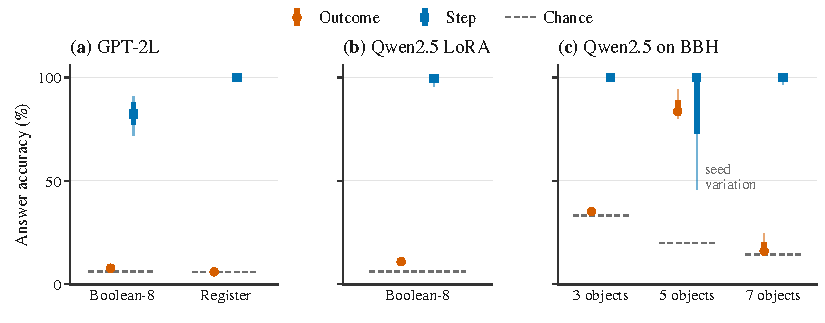
\includegraphics[width=\linewidth]{figures/main_transfer.pdf}
\caption{\textbf{Step supervision also helps beyond counting.}
Held-out answer accuracy for (a)~GPT-2L, (b)~Qwen2.5-0.5B LoRA, and (c)~Qwen2.5-0.5B LoRA on the official $250$ BIG-Bench Hard items at each object count.
Points show medians, thick intervals the interquartile range, and thin intervals the full seed range; GPT-2L Boolean-8 uses five seeds, other groups three.
Dashed segments show chance; protocols are in \cref{app:experiments}; numerical ranges are stated below.}
\label{fig:transfer}
\end{figure}
\paragraph{Purpose.} Synthetic state-tracking tasks test how degree structure relates to the supervision gap;
pretrained models and BIG-Bench Hard test whether the qualitative pattern transfers to a different setting.

\paragraph{Synthetic state tracking.} Boolean-8 has $4$ bits ($K=16$) and NOT, CNOT, SWAP and Toffoli gates on random wires ($n=8$); the register
machine has $(x,y)\in\mathbb Z_{17}^2$, five instructions, $n=16$ and answer $x$. Their answers put $98.9\%$ and $99.9\%$ of their
variance at degrees $\ge2$, while first occurrence keeps a degree-$1$ part at every $n$ (there $\mathbf 1[y=1]=b_1$, so $\E\|(\bm y-\bm u)_{\{1\}}\|^2\ge p(1-p)$). GPT-2L uses character tokens. \paragraph{Pretrained models and BIG-Bench Hard.} The LoRA runs test transfer of the qualitative mechanism beyond the controlled model.
On Boolean-8, giving Qwen2.5 eight times the outcome budget yields $10.0\pm0.9\%$ accuracy (mean$\pm$SD over seeds).
Answer-first controls give $8.0\pm0.9\%$ for GPT-2L and $10.1\pm1.0\%$ for Qwen2.5, so they do not reproduce the step benefit.



\noindent\begin{minipage}{\linewidth}
\emph{Benchmark setup and results.} Training items come from the benchmark's templates with new assignments and swaps; testing uses
the official $250$ items per size, all of which parse and rebuild exactly. Traces list every holder's item with its
option letter (``Alice has Ulysses (A)''); with item names alone, answers stayed at the letter base rate. With $m$
objects a random swap gives $\mixrate=\frac{mp-1}{m-1}$ with $p=\frac{\binom{m-1}{2}}{\binom{m}{2}}$, which is $0$, $\tfrac{1}{2}$ and $\tfrac{2}{3}$ for $m=3,5,7$, and the
share of answer variance at degrees $\le1$ is $\mixrate^{2n}+n\mixrate^{2(n-1)}(1-\mixrate^2)$: $0$, $1.56\%$ and $3.34\%$. Zero-shot accuracy is
$33.6$, $16.4$ and $11.2\%$. At three objects, outcome runs select the most common option, whose base rate is $35.2\%$.
Five objects reverse the ordering that the low-degree share predicts: outcome training reaches $80$--$94\%$ there but
$15$--$24\%$ at seven objects, whose share is larger. One of three five-object step runs fails ($46\%$ on real items, $45\%$ on
generated ones). Five objects are therefore an exception: outcome training succeeds despite less low-degree variance than seven objects.
We treat the degree calculation as a mechanistic guide, not a complete predictor of pretrained-model optimization; these LoRA runs are outside the theorem assumptions.
\end{minipage}





%=============================================================================

For the BBH spectrum measurement, we split all $6^3$ swap sequences at fixed scene, assignment and query, using the three option
logits and the LoRA up-projection Jacobian. For every task in \cref{fig:transfer}, $\mixrate$ is the largest singular value of the averaged
move permutation on mean-zero state vectors (\cref{def:lambda} for counting).
It determines the low-degree share for counting and BBH. For Boolean-8 and the register machine, it is only the slowest of many state modes:
the single-mode estimate $\mixrate^{2n}+n\mixrate^{2(n-1)}(1-\mixrate^2)$ gives $20\%$ and $56\%$, far above the measured
$1.1\%$ and $0.08\%$ degree-$\le1$ shares.

The counting summaries use a zero readout and ten paired seeds with $8$k updates for modulo $2$ (mean accuracy, solved seeds in parentheses),
and $32$k updates with seeds $42$--$44$ for modulo $3$. BBH uses $750$ official items, $250$ per size. At $n=16$, modulo-$3$
outcome accuracy is $30$--$50\%$ versus $100\%$ for steps; first-occurrence controls
reach $71$--$100\%$ versus $80$--$99\%$. BBH three-object step accuracy is
$98.4$--$100\%$ versus $35.2\%$ for outcomes; at seven objects it is
$96.4$--$100\%$ versus $15.2$--$24.4\%$. The five-object reversal and failure
are documented above.



%=============================================================================
\subsection{Joint routing runs}
\label{app:reach}

\Cref{tab:reach} uses the two-block architecture of \cref{app:model}, $K=2,p=1/4$,
full-batch gradient descent of step size $2$, $4{,}096$ training prompts and $16{,}384$
held-out prompts. Fan-in weights, embeddings of variance $1/d_{\mathrm{res}}$ and
MLP biases of magnitude $1$--$2$ are scaled by $\varepsilon=0.3$; readout and relative
biases start at zero. Only QK, relative biases and readout train. Success means every
held-out state has positive margin. The remaining $n=12$ run reaches $99.95\%$ by
$300$k updates; matched outcome runs solve none. Per-run measurements are in the repository.

%=============================================================================
\subsection{An attracting outcome trap and its initialization diagnostic}
\label{app:two-path}
We prove \cref{prop:two-path-trap} for the family \cref{eq:two-path-model}, then
report the paired initialization test. Routing and averaging are supplied in this family.

\paragraph{Expressibility check.}
The step executor takes $a=0$, $g=20$, $q=k=5$, and $v_i=0$.
For the outcome executor, take $a=g=0$, $M=n+2$, and
\[
\begin{aligned}
 f_{\mathrm{out}}(S,u)&=20\sum_{j=0}^n\sum_{r\in\{-1,1\}}r(-1)^j
 \bigl[\relu(z_{j,r}+1)-2\relu(z_{j,r})+\relu(z_{j,r}-1)\bigr],\\
 z_{j,r}&=nu-j+M(rS-1).
\end{aligned}
\]
For integer $nu$, the bracket is $1$ exactly when $j=nu$ and $r=S$, and
$0$ otherwise. Hence $f_{\mathrm{out}}=20S(-1)^{nu}$.
Unlike the one-letter predictor in \cref{lem:binary-loss-mixture}, this family
contains a count-reading path, so \cref{eq:binary-loss-mixture} does not apply to
its full loss. Executor enumeration and a counterexample are in the audit files.

\paragraph{Suboptimal local minimum.}
Let $h=\lambda^{n-1}$ be the hidden-letter correlation, and $m_{\mathrm{trap}}=\log((1+h)/(1-h))$. Construct a point with
\[
\begin{aligned}
 a&=0,\quad q=k=1,\quad g=m_{\mathrm{trap}}/\tanh(1),\quad v_i=d_i=0,\\
 (w_1,b_1)&=(1,2),\qquad (w_2,b_2)=(0,1).
\end{aligned}
\]
All remaining units have $(w_i,b_i)=(0,-1)$. Every preactivation is bounded
away from zero on $S\in\{-1,1\}$, $u\in[0,1]$. In an open parameter neighborhood,
exactly the first two units stay active, and
\[
\begin{aligned}
 f_P&=A S+B SC+D u+E,\\
 A&=a+\sum_{i=1}^2v_i d_i,\qquad B=g\tanh(qk),\\
 D&=\sum_{i=1}^2v_i w_i,\qquad E=\sum_{i=1}^2v_i b_i.
\end{aligned}
\]
Here $A,B,D,E$ are the state, state--letter, count and constant coefficients.
Let $F(A,B,D,E)$ be their outcome loss.
It is convex as a positive weighted sum of logistic losses. At
$(A,B,D,E)=(0,m_{\mathrm{trap}},0,0)$, independence of the hidden bits gives
\[
 \E[Y\mid S,C]=hSC,
 \qquad \frac{1}{1+e^{-m_{\mathrm{trap}}SC}}=\frac{1+hSC}{2}.
\]
Thus the expected logit derivative conditional on $(S,C)$ is zero, so
$\frac{\partial F}{\partial A}=\frac{\partial F}{\partial B}=0$.
The transformation $(S,Y)\mapsto(-S,-Y)$ preserves the data distribution,
fixes $(C,u)$, and reverses the logit derivative at $f=m_{\mathrm{trap}}SC$.
Consequently $\frac{\partial F}{\partial D}=\frac{\partial F}{\partial E}=0$ as well.
Convexity gives
\begin{equation}
 F(A,B,D,E)\ge F(0,m_{\mathrm{trap}},0,0)
 =-\frac{1+h}{2}\log\frac{1+h}{2}
  -\frac{1-h}{2}\log\frac{1-h}{2}>0.
 \label{eq:two-path-local-loss}
\end{equation}
This is a local minimum in the original parameters, with zero full gradient.
It is non-strict because different parameter settings realize the same logits.
Since $\operatorname{sign}(f_{\mathrm{trap}})=SC$, its accuracy is $(1+h)/2$.
Scaling the outcome executor's readout sends the global loss to zero.

\paragraph{A local trajectory invariant.}
Let $P_{\mathrm{trap}}$ be the constructed point, and define the coefficient map
$\operatorname{coeff}(P)=(A,B,D,E)$. At $P_{\mathrm{trap}}$ the columns of
$\frac{\partial\operatorname{coeff}}{\partial P}$ indexed by $a,g,v_1,v_2$ are
\[
 (1,0,0,0)^\top,\quad(0,\tanh(1),0,0)^\top,
 \quad(0,0,1,2)^\top,\quad(0,0,0,1)^\top.
\]
They span $\R^4$. The feature vectors $(S,SC,u,1)$ also span $\R^4$:
flipping $S$ in a zero linear combination forces the first two coefficients
to vanish, and two distinct values of $u$ force the last two to vanish.
Every input has positive probability. Therefore
\[
 \nabla^2 F(\operatorname{coeff})
 =\E\left[\frac{e^{f}}{(1+e^{f})^2}
 (S,SC,u,1)^\top(S,SC,u,1)\right]\succ0.
\]
By continuity, choose a closed parameter ball of radius $r$ about $P_{\mathrm{trap}}$
inside the fixed-pattern region. On this ball the coefficient Jacobian has
smallest row singular value at least $c_{\mathrm{map}}>0$; on a coefficient ball containing
its image and $\operatorname{coeff}(P_{\mathrm{trap}})$, the Hessian of $F$ is at least $c_{\mathrm{loss}} I$, $c_{\mathrm{loss}}>0$.
Strong convexity and the chain rule give, throughout the parameter ball,
\begin{equation}
\begin{aligned}
 \|\nabla_P L\|^2&\ge c_{\mathrm{map}}^2\|\nabla F\|^2
 \ge 2c_{\mathrm{map}}^2c_{\mathrm{loss}}\bigl(L-L_{\mathrm{trap}}\bigr),\\
 L_{\mathrm{trap}}&=F(0,m_{\mathrm{trap}},0,0).
\end{aligned}
 \label{eq:two-path-local-gradient}
\end{equation}
For Euclidean gradient flow, define the loss gap $G(t)=L(P(t))-L_{\mathrm{trap}}$.
Until a first exit, $\frac{dG}{dt}=-\|\nabla_P L\|^2$, hence
\[
\begin{aligned}
 G(t)&\le G(0)e^{-2c_{\mathrm{map}}^2c_{\mathrm{loss}} t},\\
 \int_0^t\left\|\frac{dP}{dt}\right\|\,dt
 &\le\frac{\sqrt{2G(0)}}{c_{\mathrm{map}}\sqrt{c_{\mathrm{loss}}}}.
\end{aligned}
\]
The second bound follows by integrating
$c_{\mathrm{map}}\sqrt{2c_{\mathrm{loss}} G}\,\|\nabla_P L\|\le-\frac{dG}{dt}$;
if $G$ reaches zero the flow is stationary.
Choose initial points satisfying
\begin{equation}
 \|P(0)-P_{\mathrm{trap}}\|<r/2,
 \qquad \frac{\sqrt{2G(0)}}{c_{\mathrm{map}}\sqrt{c_{\mathrm{loss}}}}<r/2.
 \label{eq:two-path-basin}
\end{equation}
These strict conditions contain an open neighborhood of $P_{\mathrm{trap}}$.
A first exit would require displacement at least $r/2$, contradicting
the path-length bound. The flow thus remains in a compact smooth region,
extends for all time, and has finite total length.
It converges to $P_{\mathrm{end}}$ with $L(P_{\mathrm{end}})=L_{\mathrm{trap}}$.
Strict convexity forces $\operatorname{coeff}(P_{\mathrm{end}})=(0,m_{\mathrm{trap}},0,0)$, proving the proposition.

\paragraph{Zero-readout geometry certificate.}
\label{app:random-trap-certificate}
We prove \cref{prop:random-outcome-trap}. Let $W=6(n+1)$ and write
$Z_i(S,u)=w_i u+d_iS+b_i$ at the seed $P_0$.
Require that, for each unit, the four values at $S=\pm1$, $u=0,1$ have the same
nonzero sign. Their minimum absolute value is $b_{\mathrm{margin}}>0$.
Choose two active units $i,j$ whose matrix
\[
 \begin{pmatrix}w_i&w_j\\b_i&b_j\end{pmatrix}
\]
has smallest singular value $s_{\mathrm{pair}}>0$, and require $|q_0|,|k_0|>0$. Set
\[
 r=\min\left\{\frac{b_{\mathrm{margin}}}{4\sqrt3},
 \frac{|q_0|}{4},\frac{|k_0|}{4},\frac{s_{\mathrm{pair}}}{4},1\right\},
 \qquad d_{\mathrm{pair}}=(d_i^2+d_j^2)^{1/2}.
\]
Within the closed radius-$r$ parameter ball, activation values change by at most
$\sqrt3r$, the selected feature matrix changes by at most $r$ in operator norm,
and neither query--key scalar crosses zero. The columns of the coefficient
Jacobian indexed by $a,g,v_i,v_j$ are therefore
\[
 \begin{pmatrix}
 1&0&d_i&d_j\\0&\tanh(qk)&0&0\\0&0&w_i&w_j\\0&0&b_i&b_j
 \end{pmatrix}.
\]
Solving this triangular system gives the uniform bound
\begin{equation}
 c_{\mathrm{map}}=
 \min\left\{\frac1{\sqrt2},
 \tanh\bigl((|q_0|-r)(|k_0|-r)\bigr),
 \frac{s_{\mathrm{pair}}-r}{\sqrt{1+2(d_{\mathrm{pair}}+r)^2}}\right\}>0.
 \label{eq:random-trap-map}
\end{equation}
Specifically, the squared norm of the inverse applied to a coefficient vector
is at most the maximum of $2$, $1/\tanh^2(qk)$ and
$(1+2\|(d_i,d_j)\|^2)/s^2$ times its squared norm, where $s$ is the
current pair matrix's smallest singular value. The full Jacobian can only have
a larger smallest row singular value.

Let $H_{\mathrm{seed}}$ be the maximum Euclidean norm of the seed's ReLU feature
vector at those four endpoints. Put
\[
 M=\max\left\{2r+rH_{\mathrm{seed}}+\sqrt3r^2,
                \log\frac{1-p}{p}\right\}.
\]
The first term bounds every logit in the parameter ball: $|a|,|g|,\|v\|\le r$
and the feature norm is at most $H_{\mathrm{seed}}+\sqrt3r$.
The second bounds the optimal logits, since $\lambda^{n-1}\le1-2p$.
The same bound holds on the convex hull of these coefficient vectors and the optimum.
For $X=(S,SC,u,1)$, uniform $S$ makes the two diagonal blocks of $\E[X^\top X]$
\[
 \begin{pmatrix}1&\lambda\\\lambda&1\end{pmatrix},\qquad
 \begin{pmatrix}p^2+p(1-p)/n&p\\p&1\end{pmatrix}.
\]
The first has minimum eigenvalue $2p$. The second has determinant $p(1-p)/n$
and trace at most $2$, so its minimum eigenvalue is at least $p(1-p)/(2n)$.
The logistic curvature on $[-M,M]$ is at least $(2+2\cosh M)^{-1}$. Thus
\begin{equation}
 c_{\mathrm{loss}}=\frac{p(1-p)}{2n(2+2\cosh M)}
 \quad\text{satisfies}\quad \nabla^2F\succeq c_{\mathrm{loss}}I.
 \label{eq:random-trap-loss}
\end{equation}

\paragraph{Small gap and trajectory invariant.}
Put $h=\lambda^{n-1}$. Zero readout gives $L(P_0)=\log2$, and
\cref{eq:two-path-local-loss} gives the floor $L_{\mathrm{trap}}$ throughout the ball.
The initial gap obeys
\[
\begin{aligned}
 G(0)&=\log2-L_{\mathrm{trap}}
 =D_{\mathrm{KL}}\left(\operatorname{Bern}\left(\frac{1+h}{2}\right)
                 \middle\|\operatorname{Bern}\left(\frac12\right)\right)\\
 &\le\log(1+h^2)\le h^2,
\end{aligned}
\]
where the first inequality is Jensen's inequality applied to the log density ratio.
The coefficient gradient bound and chain rule give
$\|\nabla_P L\|^2\ge2c_{\mathrm{map}}^2c_{\mathrm{loss}}G$ before a first exit.
The path-length calculation above yields
\begin{equation}
 \int_0^t\left\|\frac{dP}{dt}\right\|dt
 \le\frac{\sqrt{2G(0)}}{c_{\mathrm{map}}\sqrt{c_{\mathrm{loss}}}}
 \le\frac{\sqrt2h}{c_{\mathrm{map}}\sqrt{c_{\mathrm{loss}}}}<r/2.
 \label{eq:random-trap-path}
\end{equation}
A first exit requires length at least $r$, a contradiction.
Compact smooth continuation and finite path length give convergence of the full
parameter vector. The loss gap decays exponentially to zero; strict convexity
identifies the limiting coefficients as $(0,m_{\mathrm{trap}},0,0)$.
The limiting point is a local minimum because the uniform activation pattern
still has a positive margin. This proves \cref{prop:random-outcome-trap}.
The averaging path is not frozen by symmetry: at zero readout an active unit has
\[
 \left.\frac{\partial L}{\partial v_i}\right|_{P_0}
 =-\frac{d_i\lambda^n}{2}.
\]
Thus nonzero state weights produce an averaging-readout update. The proof controls
its total path rather than setting its gradients to zero.

\paragraph{A probability bound for the experimental initialization law.}
\begin{corollary}[Gaussian feature geometry]
\label{cor:random-trap-geometry}
Use the zero-readout initialization of the paired diagnostic, $a=g=v_i=0$, with $0<\varepsilon\le1$,
independent $w_i,d_i\sim N(0,\varepsilon^2/50)$, independently signed
$b_i$ with magnitudes uniform on $[\varepsilon,2\varepsilon]$, and independently
signed $q_0,k_0$ with magnitudes in $[\varepsilon/2,2\varepsilon]$.
Let $\Phi$ be the standard normal cumulative distribution function and put
\[
 a_{\mathrm{prob}}=\frac12\left[\Phi(\sqrt2)-\Phi(1/\sqrt2)\right],
 \qquad r=\frac\varepsilon{60}.
\]
With probability at least
\begin{equation}
 1-4W\bigl[1-\Phi(15/4)\bigr]-2(1-a_{\mathrm{prob}})^W,
 \label{eq:random-trap-probability}
\end{equation}
there is uniform fixed-pattern geometry with
$c_{\mathrm{map}}\ge\varepsilon^2/40$ and \cref{eq:random-trap-loss}, using
\[
 M=\max\left\{\log\frac{1-p}{p},
 \frac\varepsilon{30}+\frac{11\varepsilon^2\sqrt W}{240}
                   +\frac{\sqrt3\varepsilon^2}{3600}\right\}.
\]
On this event, the outcome trap follows whenever
\begin{equation}
 \lambda^{n-1}\sqrt n
 <\frac{\varepsilon^3}{9600}
   \sqrt{\frac{p(1-p)}{2+2\cosh M}}.
 \label{eq:random-trap-horizon}
\end{equation}
The probability bound is useful where its right-hand side is positive;
no width-independent asymptotic high-probability claim is made.
\end{corollary}
\begin{proof}
For independent $w_i,d_i$, the variables $w_i+d_i$ and $w_i-d_i$ have variance
$\varepsilon^2/25$, and $|w_i|+|d_i|=\max(|w_i+d_i|,|w_i-d_i|)$.
A union bound gives $|w_i|+|d_i|\le3\varepsilon/4$ for every unit except with
probability at most $4W[1-\Phi(15/4)]$. On this event the activation margin is
at least $\varepsilon/4$ and $H_{\mathrm{seed}}\le11\varepsilon\sqrt W/4$.
Each unit independently has probability $a_{\mathrm{prob}}$ of satisfying
$b_i>0$, $w_i\in[\varepsilon/10,\varepsilon/5]$, and the same probability with
$w_i\in[-\varepsilon/5,-\varepsilon/10]$.
Except with probability $2(1-a_{\mathrm{prob}})^W$, both types occur.
Their selected feature matrix has determinant magnitude at least
$\varepsilon^2/5$ and Frobenius norm at most $\sqrt{202}\varepsilon/5$;
hence $s_{\mathrm{pair}}\ge\varepsilon/\sqrt{202}>\varepsilon/15$.
The radius $\varepsilon/60$ preserves all these bounds. In
\cref{eq:random-trap-map}, the pair term is at least $\varepsilon/40$ and the
query--key term is at least $\tanh((29\varepsilon/60)^2)\ge\varepsilon^2/40$.
This proves the geometric event and its probability bound, without assuming
independence of its constituent events. Substitution into \cref{eq:random-trap-path}
gives \cref{eq:random-trap-horizon}.
\end{proof}

\paragraph{Accuracy during the trajectory.}
The limiting accuracy is the one-letter value, but the same bound need not hold
at every time in the affine region. At $n=2,p=1/4$, the affine logits $SC+4u$
have accuracy $0.78125$, above the one-letter bound $0.75$.
The count offset selects which cells use the state-dependent prediction.
What is uniform is the loss floor and a correct-answer probability bound:
by \cref{eq:random-trap-path} and the $1/4$-Lipschitz sigmoid,
\[
 \E\left[\frac1{1+e^{-Yf}}\right]
 \le\frac12+
 \frac{(2+H_{\mathrm{seed}}+\sqrt3r)\sqrt2h}
      {4c_{\mathrm{map}}\sqrt{c_{\mathrm{loss}}}}.
\]
No affine point can have positive margins on every input: scaling all its readouts
would otherwise send its loss to zero without changing the activation pattern,
contradicting the strictly positive affine loss floor.

\begin{proposition}[Process learning versus permanent outcome failure]
\label{prop:two-path-matched}
In \cref{eq:two-path-model}, let $n\ge2$, $0<p<1/2$, $0<\varepsilon\le1$,
with a uniform start, and take the common seed
\[
 a=g=v_i=d_i=0,\quad q=k=\varepsilon,\quad
 (w_1,b_1)=(\varepsilon,2\varepsilon),\quad (w_2,b_2)=(0,\varepsilon),
\]
with $(w_i,b_i)=(0,-\varepsilon)$ for $i\ge3$.
Train all parameters by population Euclidean gradient flow under each objective.
Writing $H=\log((1-p)/p)$, process flow has all transition margins at least $1$
for every time after
\[
 T\le \frac{(H+1)(1+e^{2H+1})}{\tanh^2(\varepsilon^2)}
 =O\bigl(\varepsilon^{-4}p^{-2}(1+\log(1/p))\bigr).
\]
Outcome flow converges to a suboptimal local minimum with logits
$f_{\mathrm{trap}}$ of \cref{prop:two-path-trap}; at every time its accuracy is
at most $(1+\lambda^{n-1})/2<1$.
\end{proposition}

\paragraph{Matched two-path flows.}
\label{app:two-path-matched}
We prove \cref{prop:two-path-matched}. The averaging seed has exactly two active
units, with features $\varepsilon(u+2)$ and $\varepsilon$.
At any point with $v_i=d_i=0$ and these fixed $(w_i,b_i)$, flipping the uniform
start flips $(S,Y)$, preserves all bits and $u$, and negates the logit $f$.
The logit derivative $-Y/(1+e^{Yf})$ changes sign, so
\[
 \frac{\partial L}{\partial v_i}
 =\E\left[\frac{-Y}{1+e^{Yf}}\relu(w_i u+b_i)\right]=0.
\]
All derivatives with respect to $w_i,d_i,b_i$ contain a factor $v_i$ and are zero.
This holds under both objectives and at every teacher-forced transition.
Uniqueness of the smooth flow makes this subspace invariant. Hence
$f=S(a+cC)$, with $c=g\tanh(qk)$, for all time.

For process labels take $h=1$; for outcome labels take $h=\lambda^{n-1}$.
Define
\[
 \ell_h(x)=\frac{1+h}{2}\ell(x)+\frac{1-h}{2}\ell(-x),\qquad
 F_h(a,c)=(1-p)\ell_h(a+c)+p\ell_h(c-a).
\]
The full parameter flow reduces exactly to the same system with $T=\tanh(qk)$:
\begin{equation}
\begin{aligned}
 \frac{da}{dt}&=-\frac{\partial F_h}{\partial a},&
 \frac{dg}{dt}&=-T\frac{\partial F_h}{\partial c},\\
 \frac{dq}{dt}&=-gk(1-T^2)\frac{\partial F_h}{\partial c},&
 \frac{dk}{dt}&=-gq(1-T^2)\frac{\partial F_h}{\partial c}.
\end{aligned}
\label{eq:two-path-common-flow}
\end{equation}
The initial equality $q=k$ is invariant. Direct differentiation gives
\begin{equation}
 g^2=\int_\varepsilon^q\frac{\sinh(2z^2)}{z}\,dz,
 \qquad q=k\ge\varepsilon,\qquad T\ge\tanh(\varepsilon^2)>0.
 \label{eq:two-path-factor-balance}
\end{equation}
Indeed $q$ stays positive because its differential equation has a factor $q$;
the integral is strictly increasing for $q>0$ and vanishes at $\varepsilon$.

\paragraph{Process completion.}
For $h=1$, $\partial F_1/\partial c<0$, so $g,c$ increase from zero. Moreover
\[
 \frac{da}{dt}=\frac{1-p}{1+e^{a+c}}-\frac{p}{1+e^{c-a}}.
\]
At $a=0$ this derivative is positive; at $a=H=\log((1-p)/p)$ it is nonpositive,
since for $c\ge0$
\[
 \frac{1+e^{c-H}}{1+e^{c+H}}\le e^{-H}=\frac{p}{1-p}.
\]
Thus $0\le a\le H$. The exact contrast equation is
\[
 \frac{dc}{dt}
 =\bigl[T^2+g^2(q^2+k^2)(1-T^2)^2\bigr]
 \left[\frac{1-p}{1+e^{a+c}}+\frac{p}{1+e^{c-a}}\right].
\]
Until $c=H+1$, both margins are at most $2H+1$, giving
\[
 \frac{dc}{dt}\ge\frac{\tanh^2(\varepsilon^2)}{1+e^{2H+1}}.
\]
Integrating proves the claimed time. Thereafter $c$ increases and $a\le H$, so
$c-a\ge1$ and $a+c\ge1$ persist. Finally,
$\tanh(\varepsilon^2)\ge\varepsilon^2/2$ for $0<\varepsilon\le1$ and
$e^{2H}=((1-p)/p)^2$, giving the polynomial bound.
No finite-time blow-up occurs: $|da/dt|,|dg/dt|\le1$ and
$|dq/dt|=|dk/dt|\le |g|q$ on $q=k>0$, which bounds the parameters on each finite interval.

\paragraph{Outcome convergence.}
For $h=\lambda^{n-1}\in(0,1)$, the strictly convex effective loss has its unique
minimum at
\[
 a=0,\qquad c=\log\frac{1+h}{1-h}.
\]
Let $p_{\mathrm{noise}}=(1-h)/2>0$. Since
$\ell_h(x)\ge p_{\mathrm{noise}}|x|$, loss descent from $F_h(0,0)=\log2$ yields
\[
 p_{\mathrm{noise}}p(|a|+|c|)\le F_h(a,c)\le\log2.
\]
Thus $a,c$ stay bounded. Equation~\eqref{eq:two-path-factor-balance} bounds
$|g|\le |c|/\tanh(\varepsilon^2)$ and then bounds $q=k$, because its integral
tends to infinity. The full trajectory stays in a compact smooth region.
On a convex coefficient neighborhood containing this loss sublevel,
$\nabla^2F_h\succeq c_{\mathrm{loss}}I$ for some $c_{\mathrm{loss}}>0$.
The $a,g$ coordinates of the full gradient alone give
\[
\begin{aligned}
 \|\nabla_P L\|^2
 &\ge \left|\frac{\partial F_h}{\partial a}\right|^2
       +T^2\left|\frac{\partial F_h}{\partial c}\right|^2\\
 &\ge 2c_{\mathrm{loss}}\tanh^2(\varepsilon^2)
       \bigl(F_h-\min F_h\bigr).
\end{aligned}
\]
The loss gap therefore decays exponentially. Applying the path-length calculation
of \cref{eq:two-path-local-gradient} with
$c_{\mathrm{map}}=\tanh(\varepsilon^2)$ gives finite total parameter path length.
The full flow converges, and strict convexity identifies its limiting logits as
$f_{\mathrm{trap}}$. Its uniformly active/inactive averaging units realize affine
coefficients as in \cref{eq:two-path-local-loss}, so the limit is a local minimum
of the full family. For every time, conditioning on $(S,C)$ bounds any predictor's
accuracy by $(1+h)/2$, proving permanent failure to learn the exact count.

\paragraph{Paired initialization test.}
We independently implement the population loss and its derivatives, enumerate all
inputs, and combine identical feature rows with their exact probabilities.
We use $p=1/4$, uniform $s_0$, gradient descent with step size $1$, and seeds $0,1,2$
at each $n=4,6,8$. The two initializations share $\varepsilon=0.3$, zero $a,g,v$,
and independently signed $q,k$ with magnitudes uniform on
$[\varepsilon/2,2\varepsilon]$.
The fixed-pattern initialization has independent
$w_i,d_i\sim N(0,0.02\varepsilon^2)$ and signed bias magnitudes uniform on
$[\varepsilon,2\varepsilon]$.
The alternative puts kinks in range using independent
$w_i\sim N(0,9\varepsilon^2)$, $d_i\sim N(0,\varepsilon^2)$ and
$b_i\sim N(0,0.01\varepsilon^2)$.
These are controlled initialization laws, not a standard fan-in Transformer initialization.

All nine fixed-pattern step runs attain positive margins in $11$--$15$ updates.
Fixed-pattern outcome runs end at accuracy
$(1+\lambda^{n-1})/2$, namely $0.5625$, $0.515625$, and $0.50390625$.
The caps are $60$k updates at $n=4$ and $20$k at $n=6,8$; no activation signs
change at the endpoints $u=0,1$, $S=\pm1$ during these runs.
In the alternative initialization, all nine outcome runs first cross $90\%$
accuracy within $28$--$738$ updates. This is not persistent convergence:
at the $3$k-update cap the $n=8$ runs have accuracy $68.4\%$, $83.9\%$, and $83.9\%$.
\Cref{fig:two-path-init} separates first crossings from capped accuracy.

\begin{figure}[htbp]
\centering
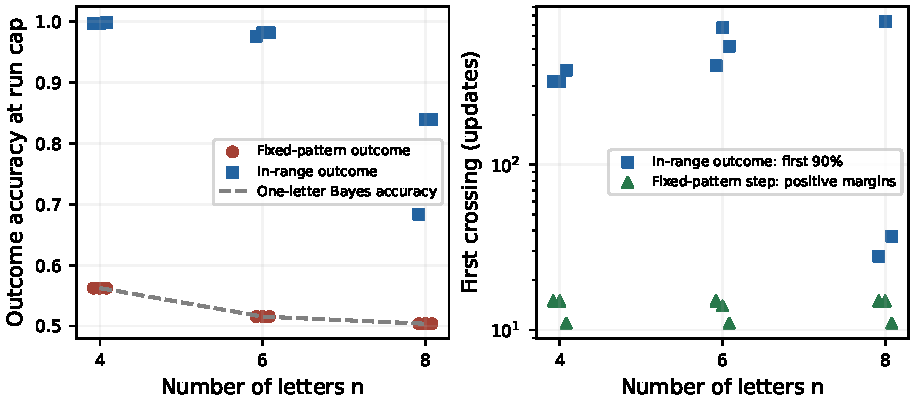
\includegraphics[width=\linewidth]{figures/two_path_initialization.pdf}
\caption{\textbf{Supplied averaging exposes an initialization boundary.}
Left: capped outcome accuracy for each paired seed; the dashed line is the
one-letter predictor's Bayes accuracy. Right: first $90\%$-accuracy crossings
for outcome training with in-range kinks and first positive margins for
fixed-pattern step training. Crossings do not assert sustained accuracy.
All runs use binary counting, population gradient descent and step size $1$.}
\label{fig:two-path-init}
\end{figure}

\paragraph{What remains unproved.}
The small-gap certificate of \cref{prop:random-outcome-trap} permits nonzero
state weights. It first passes at horizons $17,17,16$ in the three scanned seed
streams; the $n=4,6,8$ experimental seeds fail its path-length test.
The finite runs do not prove that those trajectories stay affine forever,
converge to the trap, or satisfy the matched guarantee of \cref{prop:two-path-matched}.
The process-convergence proof still covers $d_i=0$ exactly. A matched process
guarantee from the nonsymmetric seeds of \cref{prop:random-outcome-trap} remains
open. The conditional certificate and horizon scan are retained with the audit files.
The reduced experiment does not replace
\cref{thm:outcome-end}; no modulo-$3$ trap claim is made.
The independent implementation, complete trajectories at recorded checkpoints,
executor checks and identity counterexample are retained in
\nolinkurl{Paper/research/two_path/}.

%=============================================================================
\section{Reproducibility}
\label{app:reproducibility}

% TODO before submission: confirm the anonymous repository URL.
\paragraph{Code.} Code, configurations, seeds, reproduction commands, numerical proof checks and per-run measurements are available at
\url{https://anonymous.4open.science/r/trace}. The accompanying code repository provides an exact implementation of the executors,
numerical checks of the credit and plateau identities, the reduced two-path executors and attracting minimum, and instructions for reproducing the experiments.

\paragraph{Compute and data.} Runs use one NVIDIA A100 80GB GPU: about one minute per $8$k counting updates and fifteen minutes per
$800$-update LoRA run; exploratory runs used more compute than reported. Data are synthetic; the accompanying code repository also
contains the official BIG-Bench Hard items, unchanged. Software and assets: PyTorch 2.13 (BSD-3-Clause), Transformers 5.16 and PEFT 0.20 (Apache-2.0), Qwen2.5-0.5B \citep{qwen2025qwen25} (Apache-2.0), and BIG-Bench Hard \citep{suzgun2022challenging} (MIT).

